%%%%%%%%%%%%%%%%%%%%%%%%%%%%%%%%%%%%%%%%%
% Masters/Doctoral Thesis 
% LaTeX Template
% Version 1.43 (17/5/14)
%
% This template has been downloaded from:
% http://www.LaTeXTemplates.com
%
% Original authors:
% Steven Gunn 
% http://users.ecs.soton.ac.uk/srg/softwaretools/document/templates/
% and
% Sunil Patel
% http://www.sunilpatel.co.uk/thesis-template/
%
% License:
% CC BY-NC-SA 3.0 (http://creativecommons.org/licenses/by-nc-sa/3.0/)
%
% Note:
% Make sure to edit document variables in the Thesis.cls file
%
%%%%%%%%%%%%%%%%%%%%%%%%%%%%%%%%%%%%%%%%%

%----------------------------------------------------------------------------------------
%	PACKAGES AND OTHER DOCUMENT CONFIGURATIONS
%----------------------------------------------------------------------------------------

\documentclass[11pt, oneside]{Thesis} % The default font size and one-sided printing (no margin offsets)

\graphicspath{{Pictures/}} % Specifies the directory where pictures are stored

\usepackage[square, numbers, comma, sort&compress]{natbib} % Use the natbib reference package - read up on this to edit the reference style; if you want text (e.g. Smith et al., 2012) for the in-text references (instead of numbers), remove 'numbers' 
%\hypersetup{urlcolor=black, colorlinks=false} % Colors hyperlinks in blue - change to black if annoying

\usepackage{xcolor}
\hypersetup{
    colorlinks,
    linkcolor={red!0!black},
    citecolor={blue!0!black},
    urlcolor={blue!0!black}
}
\title{\ttitle} % Defines the thesis title - don't touch this

\begin{document}

\frontmatter % Use roman page numbering style (i, ii, iii, iv...) for the pre-content pages

\setstretch{1.3} % Line spacing of 1.3

% Define the page headers using the FancyHdr package and set up for one-sided printing
\fancyhead{} % Clears all page headers and footers
\rhead{\thepage} % Sets the right side header to show the page number
\lhead{} % Clears the left side page header

\pagestyle{fancy} % Finally, use the "fancy" page style to implement the FancyHdr headers

\newcommand{\HRule}{\rule{\linewidth}{0.5mm}} % New command to make the lines in the title page

% PDF meta-data
\hypersetup{pdftitle={\ttitle}}
\hypersetup{pdfsubject=\subjectname}
\hypersetup{pdfauthor=\authornames}
\hypersetup{pdfkeywords=\keywordnames}

%----------------------------------------------------------------------------------------
%	TITLE PAGE
%----------------------------------------------------------------------------------------

\begin{titlepage}
\begin{center}

\textsc{\LARGE \univname}\\[1.5cm] % University name
\textsc{\Large Doctoral Thesis}\\[0.5cm] % Thesis type

\HRule \\[0.4cm] % Horizontal line
{\huge \bfseries \ttitle}\\[0.4cm] % Thesis title
\HRule \\[1.5cm] % Horizontal line
 
\begin{minipage}{0.4\textwidth}
\begin{flushleft} \large
\emph{Author:}\\
\href{http://www.johnsmith.com}{\authornames} % Author name - remove the \href bracket to remove the link
\end{flushleft}
\end{minipage}
\begin{minipage}{0.4\textwidth}
\begin{flushright} \large
\emph{Supervisor:} \\
\href{http://www.jamessmith.com}{\supname} % Supervisor name - remove the \href bracket to remove the link  
\end{flushright}
\end{minipage}\\[3cm]
 
\large \textit{A thesis submitted in fulfilment of the requirements\\ for the degree of \degreename}\\[0.3cm] % University requirement text
\textit{in the}\\[0.4cm]
\groupname\\\deptname\\[2cm] % Research group name and department name
 
{\large \today}\\[4cm] % Date
%\includegraphics{Logo} % University/department logo - uncomment to place it
 
\vfill
\end{center}

\end{titlepage}


%----------------------------------------------------------------------------------------
%	QUOTATION PAGE
%----------------------------------------------------------------------------------------

\pagestyle{empty} % No headers or footers for the following pages

\null\vfill % Add some space to move the quote down the page a bit

\textit{``Thanks to my solid academic training, today I can write hundreds of words on virtually any topic without possessing a shred of information, which is how I got a good job in journalism."}

\begin{flushright}
Dave Barry
\end{flushright}

\vfill\vfill\vfill\vfill\vfill\vfill\null % Add some space at the bottom to position the quote just right

\clearpage % Start a new page

%----------------------------------------------------------------------------------------
%	ABSTRACT PAGE
%----------------------------------------------------------------------------------------

\addtotoc{Abstract} % Add the "Abstract" page entry to the Contents

\abstract{\addtocontents{toc}{\vspace{1em}} % Add a gap in the Contents, for aesthetics

The Thesis Abstract is written here (and usually kept to just this page). The page is kept centered vertically so can expand into the blank space above the title too\ldots
}

\clearpage % Start a new page

%----------------------------------------------------------------------------------------
%	ACKNOWLEDGEMENTS
%----------------------------------------------------------------------------------------

\setstretch{1.3} % Reset the line-spacing to 1.3 for body text (if it has changed)

\acknowledgements{\addtocontents{toc}{\vspace{1em}} % Add a gap in the Contents, for aesthetics

The acknowledgements and the people to thank go here, don't forget to include your project advisor\ldots
}
\clearpage % Start a new page

%----------------------------------------------------------------------------------------
%	LIST OF CONTENTS/FIGURES/TABLES PAGES
%----------------------------------------------------------------------------------------

\pagestyle{fancy} % The page style headers have been "empty" all this time, now use the "fancy" headers as defined before to bring them back

\lhead{\emph{Contents}} % Set the left side page header to "Contents"
\tableofcontents % Write out the Table of Contents

\lhead{\emph{List of Figures}} % Set the left side page header to "List of Figures"
\listoffigures % Write out the List of Figures

\lhead{\emph{List of Tables}} % Set the left side page header to "List of Tables"
\listoftables % Write out the List of Tables

%----------------------------------------------------------------------------------------
%	ABBREVIATIONS
%----------------------------------------------------------------------------------------

\clearpage % Start a new page

\setstretch{1.5} % Set the line spacing to 1.5, this makes the following tables easier to read

\lhead{\emph{Abbreviations}} % Set the left side page header to "Abbreviations"
\listofsymbols{ll} % Include a list of Abbreviations (a table of two columns)
{
\textbf{LAH} & \textbf{L}ist \textbf{A}bbreviations \textbf{H}ere \\
%\textbf{Acronym} & \textbf{W}hat (it) \textbf{S}tands \textbf{F}or \\
}


%----------------------------------------------------------------------------------------
%	DEDICATION
%----------------------------------------------------------------------------------------

\setstretch{1.3} % Return the line spacing back to 1.3

\pagestyle{empty} % Page style needs to be empty for this page

\dedicatory{For/Dedicated to/To my\ldots} % Dedication text

\addtocontents{toc}{\vspace{2em}} % Add a gap in the Contents, for aesthetics

%----------------------------------------------------------------------------------------
%	THESIS CONTENT - CHAPTERS
%----------------------------------------------------------------------------------------

\mainmatter % Begin numeric (1,2,3...) page numbering

\pagestyle{fancy} % Return the page headers back to the "fancy" style

% Include the chapters of the thesis as separate files from the Chapters folder
% Uncomment the lines as you write the chapters

% Chapter 1

\chapter{Introduction} % Main chapter title

\label{Chapter1} % For referencing the chapter elsewhere, use \ref{Chapter1} 

\lhead{Chapter 1. \emph{Introduction}} % This is for the header on each page - perhaps a shortened title

%----------------------------------------------------------------------------------------

\section{The importance of music analysis}
The incredible growth of the Web over the last pair of decades has drastically changed many of our habits. One of the areas that have been highly affected by this fast-paced growth is our consumption of multimedia contents: the use of physically-stored content is seeing itself heavily reduced, as we are more and more getting used to the access of huge databases of multimedia content through the Web.\\ (it would be nice to cite \cite{orio06} here to present the subject in a more elegant way)
Music is one of these fields that have been revolutionized by this trend: the last decade has seen the rise of several Web services (iTunes, Spotify, Pandora, Google Music just to name a few) that offer their users an easy way to access their enormous catalogue of songs. Statistics show an increasing rate of annual growth for each of these services, in both the amount of users and of revenues: now they are among the most used ways of enjoying and discovering music. \\
However, the transition to this type of services has brought to some new problems. One of them relies on the vastness of these databases: given that users want to easily discover new music suitable to their tastes through intelligently created playlists, a way to reasonably pick songs and artists among the entire catalogue is needed. \\
This, among others, has been one reason of the rapid growth of \textbf{Music Information Retrieval} (MIR), an interdisciplinary research field whose subject is to provide new ways of finding information in music. Main techniques of describing music can be grouped into two categories: 
\begin{itemize}
\item Metadata (literally \textit{data describing data}), descriptors of music not directly retrieved from the audio signal but instead from external sources \footnote{There is a lack of agreement on the use of the term \texit{metadata}, therefore its meaning could be different in other resources. For instance, it may be used to indicate all the data describing an audio file, including the ones derived from some computation on the audio signal itself.}
\item Audio content descriptors, automatically computed from audio.
\end{itemize}
When it comes to choosing one method over the other, it becomes clear that both these categories of tools have their own pros and cons. Regarding metadata, major concerns arise from the questionable consistency of the descriptors among the entire catalogue catalogue of music, given that they may have been extracted from several sources. Other concerns also arise from how well they actually describe the audio track. On the other hand, audio content descriptors (especially the low-level ones) may have no musical meaning and therefore they could be hard to understand. Many efforts have be taken in order to improve the methods of information extraction of both these categories. In general, however, audio content descriptors are thought to be more flexible, since they can be easily and equally computed for any track. One advantage of this technique relies on the fact that these kind of descriptors could easily be computed not just for each kind of song, but also for any segment inside of it. This has for example been exploited by \textit{Shazam}, a widely-used smartphone app for music identification that analyzes peaks in the frequency-time spectrum throughout all song length to build a very robust song identification system \cite{shazam03}. Another popular product that performs audio content analysis just for short segments of a song is The Infinite Jukebox\footnote{\url{http://infinitejuke.com}}, a web-application built upon Echonest library and written by Paul Lamere, that allows users to indefinitely listen to the same song, with the playback automatically jumping to points that sound very similar to the current one. The Infinite Jukebox can be considered an application of the so-called \textit{creative-MIR} \cite{xavier2013}, an emerging area of activity inner to MIR whose subject is to exploit MIR techniques for creative purposes.  Other relevant software that exploit Echonest library for similar purposes is Autocanonizer\footnote{\url{http://static.echonest.com/autocanonizer}} and Wub Machine\footnote{\url{http://thewubmachine.com}}. However, there aren't many commercial or research-based software tools that exploit this kind of techniques for creative interaction or manipulation of audio tracks at the moment. Probably the most relevant commercial system is Harmonic Mixing Tool\footnote{\url{http://www.idmt.fraunhofer.de/en/Service_Offerings/technologies/e_h/harmonic_mixing_tool.html}}, that performs audio content analysis on the user's music collection in order to allow a pleasant and harmonic fade when mixing between songs. More recently, the research-based software AutoMashUpper has been developed with the intent of automating generating multi-song mashup\footnote{A mashup is a composition made of two or more different songs playing together.} while also allowing the user a control over the music generated \cite{automash14}. WRITE MORE ABOUT AUTOMASH HERE

%----------------------------------------------------------------------------------------

\section{Phonos Project}
Phonos project\footnote{\url{http://phonos.upf.edu/}} is an initiative of the \textbf{Music Technology Group} (Universitat Pompeu Fabra, Barcelona) in collaboration with \textbf{Phonos Foundation}. Phonos was founded in 1974 by J.M. Mestres Quadreny, Andres Lewin-Richter and Luis Callejo, and for many years it has been the only studio of electroacoustic music in Spain. Many of the electroacoustic musicians in Spain attended the courses of the composer Gabriel Brncic at Phonos. It became Phonos Foundation 1982 and in 1984 it was registered at the Generalitat de Catalunya. In 1994, an agreement of co-operation with Music Technology group was established, with the purpose of promoting cultural activities related to research in the music technology. 
In 2014, an exhibition at Museum de la Musica has been planned, with the purpose of celebrating the 40th anniversary of Phonos and showing many of the instruments used in the studio, while allowing visitors to listen to the music works produced there during all these years. Given the songs' average length and their complexity, a way for the visitors to quickly and nicely explore a catalogue of songs produced in these 40 years was needed.

\begin{figure}[htbp]
  \centering
    
\includegraphics{Figures/phonos.png}
    \rule{35em}{0.5pt}
  \caption[Phonos]{Phonos Logo.}
  \label{fig:Phonos}
\end{figure}

%----------------------------------------------------------------------------------------

\section{GiantSteps}
GiantSteps\footnote{\url{http://www.giantsteps-project.eu/}} is a STREP project coordinated by JCP-Consult SAS in France in collaboration with the MTG funded by the European Commission. The aim of this project is to create the "seven-league boots" for music production in the next decade and beyond, that is, exploiting the latest fields in the field of MIR to make computer music production easier for anyone. Indeed, despite the increasing amount of software and plugins for computer music creation, it's still considered very hard to master these instruments and producing songs\footnote{ "Computer music today is like piloting a jet with all the lights turned off." (S. Jordà). \url{http://vimeo.com/28963593}} because it requires not only musical knowledge but also familiarity with the tools (both software and hardware) that the artist decide to use, and whose way of usage may greatly vary between each other. The GiantSteps project targets three different directions:
\begin{itemize}
\item Developing \textbf{musical expert agents}, that could provide suggestions from sample to song level, while guiding users lacking inspiration, technical or musical knowledge
\item Developing improved \textbf{interfaces}, implementing novel visualisation techniques that provide meaningful feedback to enable fast comprehensibility for novices and improved workflow for professionals.
\item Developing \textbf{low complexity algorithms}, so that the technologies developed can be accessible through low cost portable devices. 
\end{itemize}

Started on November 2013, GiantSteps will last 36 months and the institutions involved are:
\begin{itemize}
\item \textbf{Music Technology Group}, Universitat Pompeu Fabra, Barcelona, Spain
\item \textbf{JCP-Consult SAS}, France
\item \textbf{Johannes Kepler Universität Linz}, Austria
\item \textbf{Red Bull Music Academy}, Germany
\item \textbf{STEIM}, Amsterdam, Netherlands
\item \textbf{Reactable Systems}, Barcelona, Spain
\item \textbf{Native Instruments}, Germany
\end{itemize}

\begin{figure}[htbp]
  \centering
    
\includegraphics{Figures/giantsteps.png}
    \rule{35em}{0.5pt}
  \caption[GiantSteps]{GiantSteps Logo.}
  \label{fig:GiantSteps}
\end{figure}

%----------------------------------------------------------------------------------------

\section{Purpose of this work}
The purpose of this work is to develop a software to be used by visitors during the exhibition \textit{Phonos, 40 anys de música electrònica a Barcelona} and that allows users to easily explore a medium-sized collection of music. This software is intended to exploit latest MIR findings to create a flow of music, composed of short segments of each song, concatenated in a way that the listener can barely realize of the hops between different songs. The application developed is meant to be part of the GiantSteps and therefore should follow the three guidelines explained in the previous page.

\subsection{Structure of the dissertation}
This dissertation is organized as follows:
\begin{itemize}
\item The first part will at first give an overview regarding music analysis techniques, explaining \textit{metadata}, audio content analysis and the differences between them. Then, common techniques of music similarity computation will be explained. 
\item The second part will be about the methodology, explaining the different stages of the development, the problems faced and the techniques used. A presentation of the case study will introduce to an explanation of the reasons that lead to prefer the use of some techniques over others.
\item Finally, experimental results will be shown, together with some ideas regarding future development of the application.
\end{itemize}

%----------------------------------------------------------------------------------------

\newpage
\thispagestyle{headings}
\mbox{}
\part{Background}
\newpage
\thispagestyle{plain}
\mbox{}
\chapter{Music Analysis Techniques} 
\label{Chapter2} 

\lhead{Chapter 2. \emph{Music Analysis Techniques}} 
The main subject of MIR regards the \textit{extraction and inference of musically meaningful features, indexing of music} (through these features) and the development of \textit{search and retrieval schemes} \cite{downieMIR}. In other terms, the main target of MIR is to make all the music over the world easily accessible to the user \cite{downieMIR}. During the last two decades, several approaches have been developed, which mainly differ in the music perception category of the features they deal with. These categories generally are: \textit{music content}, \textit{music context}, \textit{user properties} and \textit{user context} \cite{gomez14}. \textit{Music content} deals with aspects that are directly inferred by the audio signal (such as melody, rhythmic structure, timbre) while \textit{music context} refers to aspects that are not directly extracted from the signal but are strictly related to it (for example label\cite{pachet00}, artist and genre information \cite{perfe11} \cite{aizenberg12}, year of release \cite{vangulik05}, lyrics \cite{coelho13} and semantic labels). Regarding the user, the difference between \textit{user context} and \textit{user properties} lies on the stability of aspects of the user himself. The former deals with aspects that are subject to frequent changes (such as mood or social context), while the latter refers to aspects that may be considered constant or slowly changing, for instance his music taste or education \cite{gomez14}. \\In this chapter, we will focus on the differences between the categories \textit{music content} and \textit{music context}. 


\section{Metadata}
By metadata we mean all the descriptors about a track that are not based on the \textit{music content}. Therefore, they are not directly extracted from the audio signal but rather from external sources. They began to be deeply studied since the early 2000s, when first doubts about an upper threshold of the performance of audio content analysis systems arised \cite{aucou04}. Researchers then started exploring the possibility of performing retrieving tasks on written data that is related to the artist or to the piece. \\At first, the techniques were adapted from the Text-IR ones, but it was immediately clear that retrieving music is fairly more complex than retrieving text, because the music retrieved should also satisfy the musical taste of the user who performed the query. 
\\The techniques used in this category may differ both in the sources used for retrieving data and in the way of computing a similarity score, and clearly the performance of a system using metadata for similarity computation is highly affected by both of these factors. Sources may include \cite{bogdanov13}:
\begin{itemize}
\item Manual annotation: description provided by experts; they may be referred to genre, mood, instrumentation, artist relations.
\item Collaborative filtering data: data indirectly provided by users of web communities, in the form of user ratings or listening behaviour information.
\item Social tags: data directly provided by users of social network of music (such as \textit{Last.fm}\footnote{\url{http://last.fm}}) or social games.
\item Information automatically mined from the Web. Sources in these cases may include web-pages related to music or microblogs (for instance the very popular \texit{Twitter}).
\end{itemize}
 The availability of some of them greatly depends on the size of the music collection under consideration; for instance, as manual expert annotations might be very accurate, they would be extremely costly and probably infeasible on large collections \cite{Szyma09}. In contrast, collaborative filtering data may be the most studied technique, given that it may be applied to other different fields (such as movies or books recommendation) with just little changes. It is the predominant approach in the field of Recommender Systems (RS) \cite{jannach12} and is mainly focused on user ratings, generally leading to better results \cite{green09}. However, some concerns are related to this technique. First, collaborative filtering approaches have not been designed to be used for playlist generation, but mainly for recommending artists or music. Second, the availibility of datasets for user ratings in the field of music is very limited compared to other fields, and research is often based on very small samples \cite{liu09}. Regarding listening behaviour information, they might be inaccurate  since they don't keep track of song durations and of the user activities while listening to music \cite{jawaheer10}. In addition, there's no way of collecting negative feedback (\textit{dislikes}) through them and, more in general, listening to a specific song doesn't necessarily imply liking that song \cite{bogdanov13}. \\Sources are picked also in relation to the subject of the research or of the system, that may be for example a recommendation or a similarity computation system. At this point, it's important to highlight the difference between the two of them: a recommendation system not only has to find similar music, but has also to take into account the personal taste of the user, and therefore it's generally considered as a basic tool to produce recommendation \cite{celma08}. In any case, the terms ``similarity'' and ``recommendation'' cannot be substituted, given that a good similarity computation system doesn't necessarily equate to a good recommendation system \cite{mcnee06}. 
 %For this kind of systems, collaborative filtering data has shown to lead to better results \cite{green09}. However, in the field of music similarity computation, social tags and keywords extracted from webpages have shown good performances. 
 The computation of similarity may happen through a Vector Space Model (a technique adapted from the Text-IR), co-occurence analysis or frequent-pattern mining. In the next subsections we will briefly explain the characteristics and the performance of these techniques.

\subsection{Vector Space Model} 
The main idea of this technique lies on building a bag-of-words representation \footnote{A bag-of-words can be basically seen as an extension of a programming language ``dictionary'': it collects words (that sometimes may just be an abstraction of much more complex features, such as computer vision descriptors) from a document, and then computes the frequency with which each of them appears in the document. Two different documents are considered similar if they contain the same or similar words with a comparable frequency.} of a retrieved document, and then computing a term weight vector for each document. It's a frequently used technique in Text-IR (and in Computer Vision) which can safely be used when retrieving web pages related to music, in an attempt of computing similarity. One of the first work in this field \cite{whitman02} provided an analysis of this kind on music-related web pages retrieved with the queries (to the \textit{Google} search engine) ``artist'' \texttt{music review} and ``artist'' \texttt{genre style}, where words such as music and review where added to improve the chances of automatically retrieving webpages related to music. 
\subsection{Co-Occurence Analysis}
\subsection{Frequent Pattern Mining}

\section{Audio Content Analysis}
The main idea behind this kind of analysis is to directly extract useful information, through some algorithms (or library of algorithms), from the audio signal itself. The type of content information extracted may greatly vary in relation to the need of the research, but we can mainly distinguish four categories \cite{bogdanov13}:
\begin{itemize}
\item \textit{Timbral} information: related to the overall quality and color of the sound.
\item \textit{Temporal} information: related to rhythmic aspects of the composition, such as tempo or length of measures.
\item \textit{Tonal} information: directly linked to the frequency analysis of the signal and to the pitch. It can describe \texit{what notes are being played} or the tonality of a given track.
\item \textit{Inferred semantic} information: information inferred (usually through machine learning techniques) from the previous categories, in the attempt of giving a more defined and understable shape to the data collected. This kind of information may include descriptors such as genre, valence or arousal.
\end{itemize}

Information extracted through this family of techniques may also be categorized in the following way:
\begin{itemize}
\item Low-level data: information that has no musical meaning and that, more in general, is not interpretable by humans. Examples of this kind of descriptors are Mel Frequency Cepstral Coefficients (MFCCs) and Zero Crossing Rate (ZCR).
\item Mid-level data: information that has musical meaning but that is related to low-level music features. This kind of category mainly includes temporal and tonal descriptors. 
\item High-level data: corresponding to inferred semantic information.
\end{itemize}

Many of the studies conducted on the computation of music similarity through audio content descriptors have solely focused on low-level and timbral information, because this has been proved to bring alone to acceptable results with proper similarity measures \cite{mirage07}. However, more recent studies have shown some evidence of advantages in using high-level descriptors \cite{barrington07} \cite{west07} and, more in general, the most performant systems use data from all of these categories. When computing low and mid-level descriptors, the procedure requires the following operations:
\begin{itemize}
\item Conversion of the signal from stereo to mono, in order to compute all the descriptors for just one signal
\item Down-sampling of the signal to improve the performance while computing the descriptors
\item Segmentation of the signal into frames, short segments (usually from 512 to 2048 audio samples). Consecutive frames are usually not disjoint: the so-called \textit{hop-size} determines the hop of samples between the beginning of a frame and the next one, and is normally half or a quarter as big as the \textit{frame size}.
\item Computation of Fast Fourier Transform, with an appropriate prior windowing technique \footnote{Although this last step may not be strictly seen as a necessary operation, many descriptors rely on frequency analysis of the signal and therefore they require the computation of the Fourier Transform.}.
\end{itemize}
The computation of descriptors is then performed on each frame, and finally a single value for each descriptor is computed by the means of some statistical analysis. Mean, median, variance and covariance are the most used statistical tools for calculating representative global values out of the enormous \textit{pool} of values computed in each frame.\\
Some more operations may sometimes be needed, such as de-noising \footnote{A set of operations which purpose is to reduce the amount of background noise in a signal, therefore incrementing the \texit{signal-to-noise ratio} (\textit{SNR} or sometimes \textit{S/N}).} of time-scaling of the signal. \\
\\In the next sections, a more detailed look among most important descriptors will be given.

\subsection{Low-level Descriptors}
\subsubsection{MFCC}


\subsection{Mid-level Descriptors}
\subsubsection{Rhythm}
In traditional music notation, there are several notations for tempo. It may be expressed in BPM (beats per minute), MPM (measures per minute; commonly used in ballroom dance music) or by semantic notations indicating a range of BPM; an example of this last category of notations may be the popular system of Italian markings, such as \textit{presto} (168-200 BPM), \textit{andante} (84-90 BPM) or \textit{allegro} (120-128 BPM). \\ In the field of MIR, accurate notations are needed, therefore semantic annotations are disregarded in favour of more precise notation such as BPM and Onset Rate (OR).
\\ \\ 
\textbf{Onset Rate} \\ 
IDEAS: image of ADSR, some flowchart for a standard onset detection algorithm (look at figures folder)
Onsets are generally defined as the beginning of a new musical note, and onset rate is therefore defined as the number of onsets in a time interval. This definition however hides several difficulties: in polyphonic music, nominally simultaneous notes may be spread over tens of seconds, making this definition more blurred \cite{dixon06}. Moreover, several instruments have a long attack time and this makes the task of defining an onset time even harder. \\Several ways of computing an onset detection function have been proposed, according to what aspects are taken into account for defining an onset. Actually, onset detection may be performed in time domain (when looking for significant changes in the overall energy), frequency domain (if looking for events regarding just a specific range of frequencies), phase domain or complex domain. 
Important algorithms for this task are:
\begin{itemize}
\item \textit{HFC}, the High Frequency Content detection function that looks for important changes on highest frequencies. It is very useful for detecting percussive events.
\item Spectral Flux, that decomposes the entire audible range of frequencies (approxitamely the interval 20-20000 Hz) into bins, measures changes in magnitude in each bin, and then sums all the positive changes across all the bins.
\item the Complex-Domain spectral difference function \cite{bello04} taking into account changes in magnitude and phase. It emphasizes note onsets either as a result of significant change in energy in the magnitude spectrum, and/or a deviation from the expected phase values in the phase spectrum, caused by a change in pitch.
\end{itemize}  
HFC was proposed by Masri in \cite{masri96}. Let us consider the short-time Fourier transform (STFT) of the signal $x(n)$:\\
\begin{equation}
X_k(n) = \sum\limits_{m=-\frac{N}{2}}^{\frac{N}{2}-1} x(nh + m)w(m)e^{-\frac{2j\pi mk}{N}}
\end{equation}
where $w(m)$ is again an $N$-point window, and $h$ is the hop size, or time shift, between adjacent windows. The idea behind HFC is to give more weight to higher frequencies, by defining a onset function whose values are computed in the follwing way:
\begin{equation}
HFC(n) = \frac{1}{N}\sum\limits_{k=-\frac{N}{2}}^{\frac{N}{2}-1} k\abs{X_k(n)}^{2}
\end{equation}

The HFC function produces sharp peaks during attack transients and is notably successful when faced with percussive onsets, where transients are well modeled as bursts of white noise \cite{bello05}.\\
On the other hand, the Spectral Flux $SF$ function is defined as follows:
\begin{equation}
SF(n) = \sum\limits_{k=-\frac{N}{2}}^{\frac{N}{2}-1} H(\abs{X(n, k)} - H(\abs{X(n - 1, k)})
\end{equation}
where $H = \frac{x + \abs{x}}{2}$ is the half-wave rectifier function. This algorithm greatly characterizes changes in magnitude spectrum but it quite weak to frequency-modulation phenomena (such as vibrato). To this end, the recently proposed variant SuperFlux \cite{bock13} seems to achieve much better results. \\
Another interesting onset function is the \textit{Complex Domain}, that calculates expected the expected amplitude and phase of the current bin $X(n, k)$ based on the previous two bins $X(n - 1, k)$ and $X(n -2, k)$. By assuming constant amplitude the expected value $X_T(n, k)$ is then computed:
\begin{equation}
X_T(n, k) = \abs{X(n - 1, k)}e^{\psi (n - 1, k) + \psi ' (n - 1, k)} 
\end{equation}
and therefore a complex domain onset detection function CD can be defined as the sum of absolute deviations from the target values \cite{dixon06}:
\begin{equation}
CD(n) = \sum\limits_{k=-\frac{N}{2}}^{\frac{N}{2}-1} \abs{X(n, k)-X_T(n,k)}
\end{equation}

Given an onset function (for instance one of the already cited $HFC(n)$, $SF(n)$ or $CD(n)$), onsets are then extracted by a peak-picking algorithm which finds local maxima in the detection function, subject to various constraints. Threshold and constraints used in the peak-picking algorithm has a large impact on the results, specifically on the ratio of false positives\footnote{True onsets that are not detected by the algorithm.} to false negatives\footnote{Points that are classified as onsets by the algorithm, while they are actually not.}. For instance, a higher threshold may lead to a lower number of false negatives but to a higher number of false positive, while a lower threshold may have the opposite effect. A compromise, mostly specific to the application, has to been found.
\\ \\ 
\textbf{BPM} \\ 
The algorithms for detecting the beats-per-minute (generally called \textit{beat tracking algorithms}) greatly rely on onset detection funcions. The basic idea is to look for some time-pattern that may explain the distribution of onsets over time, and hence derive BPM. They usually require more than one onset detection function to achieve good results. One of the most performant beat tracking algorithm is TempoTapDegara, presented by N. Degara et al. in \cite{degara12}. \\ EXPLAIN ALGORITHM HERE

\subsubsection{Tonality}
Many efforts have been taken in order to improve the techniques for detecting tonality or harmonic content of a song, as this is one of the most main aspects of western music (a direct consequence of tonality is the detection of predominant melody; to understand why this is so important just ask yourself how many times you whistled or sang a song to let other people recognize it). Many studies have focused on this aspect of music were not oriented toward the computation of similarity between tracks, but instead toward different tasks, such as \textit{automatic trascription of a polyphonic audio signal} (mainly into a MIDI representation) and \textit{source separation}, that is the task of isolating a single and specific instrument among many playing together. \\
From a music point of view, in western music, an octave is made of 12 different pitches, and seven differents notes take place in this discrete range. According to the pitch assigned to each note, we may have different \textit{keys}, that are a combination of a \textit{tonic} (the central pitch) and the mode. \textit{Major} and \textit{minor} are the most popular modes. (ADD IMAGE OF THESE TWO MODES) \\
\textit{Harmony} is a term that denotes the simultaneous combination of notes, called \textit{chords}, and over time, \textit{chord progressions}.  \\
One of the most important descriptor for extracting information related to tonality is called Harmonic Pitch Content Profile (\textbf{\textit{HPCP}}, also called chromagram). This is directly related to tonality and chord detection: chords can be recognized from from the \textit{HPCP} without even precisely detecting what notes are being played, and tonality can also be inferred by \textit{HPCP} (and in this case a previous estimation of chords is not necessary). \\
An \textit{HPCP} is a $12k$-sized vector indicating the level energy for each profile class. If $k=1$, the \textit{HPCP} represents the intensities of the twelve semitone pitch classes, otherwise of subdivision of these\footnote{It may be extremely useful to study subdivision of semitone pitch classes when dealing with non-chromatic scales, that are very popular in eastern music.}. In \cite{gomez06}, Gómez proposes to distinguish tonality features on temporal scales: 
\begin{itemize}
\item Instantaneous: features attached to an analysis frame.
\item Global: features related to a wider audio segment, for instance a phrase, a chorus or the whole song.
\end{itemize}
Furthermore, Gómez proposes to split tonal descriptors in both low-level and high-level descriptors. We hence obtain the representation of tonal descriptors shown in Table \ref{table:tonaldescriptors}.
\begin{table}[h]
\begin{center}
\begin{tabular} { l l l }
\hline
Name         & Temporal Scale & Level of abstraction \\ \hline
HPCP         & Instantaneous  & Low                  \\ 
Chord        & Instantaneous  & High                 \\ 
Average HPCP & Global         & Low                  \\ 
Key          & Global         & High                 \\ \hline
\end{tabular}
\caption{Main tonal descriptors.}
\label{table:tonaldescriptors}
\end{center}
\end{table}

The general approach for computing \textit{HPCP} is indicated in figure PUT BLOCK DIAGRAM HERE and can be summarized as follows:
\begin{itemize}
\item At first, some pre-processing of the audio signal may be performed. For instance, a transient detection algorithm may be used to detect and eliminate regions where the harmonic structure is noisy. This step is usually performed to decrease the computational cost of the \textit{HPCP} without affecting its output \cite{bonada00}.
\item At this point, spectral analysis is required: once the signal is segmented into frames of a proper size and a windowing function is applied, the Fast Fourier Transform (\textit{FFT}) is computed to get the frequency spectrum. Frames should not be too short, in order to have a better frequency resolution. 
\item A peak-picking algorithm is run to find those frequencies corresponding to local maxima in the spectrum. Usually, these algorithms are not run only on the interval [100, 5000] Hz: this has shown much better results, because outside this range the signal is predominantly noisy, due to some percussion and instrumental noise \cite{gomez06}.
\item The \textit{HPCP} is finally computed; many approaches have been developed for this task, all based on the pitch content profile algorithm presented by Fujishima in \cite{fujishima99}. At first, a mapping of each frequency bin of the \textit{FFT} to a pitch class is needed (for instance, \textit{FFT} bins corresponding to frequencies like 430Hz, 432Hz or 444Hz are mapped to the A at 440Hz). Then, the amplitudes inside each region are summed up and divided by the number of bins inside that region. Finally, the bins obtained are collapsed, so that bins referring to the same note but in a different octave (for example A4 and A5) are collapsed in a single bin for that note, indicating the overall energy of it in the frame. The \textit{HPCP} is different from the PCP in the sense that a higher resolution may be used for \textit{HPCP} bins (decreasing the quantization level to less than a semitone) and a weight function is introduced into the feature computation. The \textit{HPCP} value of the $n$-th \textit{HPCP} bin is calculated as:
\begin{equation}
HPCP(n) = \sum\limits_{i=1}^{nPeaks} w(n, f_i)a_i^2
\end{equation}
where $a_i$ and $f_i$ are respectively the magnitude and the frequency of the $i$th peak, $nPeaks$ is the number of spectral peaks considered, and $w(n, f_i)$ is the weight of the frequency bin $f_i$ when considering the \textit{HPCP} bin $n$.
\\ The performance of the \textit{HPCP} builder strongly relies on the weight function \cite{cabral05}. Note that, for how the common procedure of building \textit{HPCP} is defined, \textit{HPCP} are usually considered robust to noise and different tuning references. \\
\textit{HPCP} values are usually normalized in order to store the relative importance of the $n$th \textit{HPCP} bin:
\begin{equation}
HPCP_{normalized}(n) = \frac{HPCP(n)}{Max_n(HPCP(n))}
\end{equation}
\end{itemize}

Once the \textit{HPCP} are computed, additional tonal features may be computed, such as tonality or chords. Regarding tonality estimation, this is generally computed through a correlation analysis between the \textit{HPCP} obtained and a matrix of \textit{HPCP} profiles corresponding to different keys. 

\subsection{High-level Descriptors}

\subsection{Main Tools For Extracting Audio Content}
Many tools are available for the extraction of audio content descriptors from an audio signal. Many of them have been developed by researchers following the research necessities of MIR. This great variety of tools offers support to several operative systems (mainly Linux, Mac OS X and Windows) and programming languages (Java, C++, C, Python, Matlab). Some of this tools may be offered as standalone software or as a Vamp plugin. Not all the tools for extracting audio content are open-source, therefore not being particularly useful for the research community. In the following paragraphs, we'll briefly show the features of the tools taken into account on the development of this work.


\subsubsection*{Essentia}
Essentia\footnote{\url{http://essentia.upf.edu/}} is an open-source C++ library of algorithms for audio analysis and audio-based music information retrieval. It has been developed at Music Technology Group\footnote{\url{http://mtg.upf.edu/}}, Universitat Pompeu Fabra, and has released under the Affero GPL license\footnote{\url{http://www.gnu.org/licenses/agpl.html}}. In its current version 2.0.1, it contains a large collection of spectral, temporal, tonal, and high-level music descriptors, algorithms for audio input/output functionality, standard digital signal processing blocks and statistical tools. The library can be complemented with Gaia \footnote{\url{https://github.com/MTG/gaia}}, a C++ library to apply similarity measures and classifications on the results of audio analysis. Both these libraries include Python 2.* bindings and support Linux, Mac OS X and Windows. Essentia has been in developed for over 7 years, incorporating the work of more than 20 researchers and developers through its history. \\
It offers two different modes: standard and streaming, the first being imperative while the latter being declarative. Each processing block is offered as an algorithm, and has three different types of attributes: inputs, outputs and parameters. Different blocks may be linked in order to perform the required processing task. In figure INSERT FIGURE a block diagram of a processing task is shown, composed of several different algorithms linked together. See Appendix A for consulting the full list of descriptors provided by Essentia 2.0.1.


\subsubsection*{The Echo Nest}
\textit{The Echo Nest}\footnote{\url{http://the.echonest.com/}} is a company that provides access, through Web API, to a collection of audio descriptors for a catalogue of over 36 million songs and almost 3 million artists. In order to access to this database, an API key is required, and some rate limits are imposed to the use of a free license (for instance, the maximum number of HTTP calls for minute is subject to a limit, generally 120). Users can decide to upload their collection into this database, so that descriptors will be computed for new songs and made available to other users. The performance of this library greatly depends on the chance that a song that is about to be analyzed has already been uploaded into this service. If this is not the case, the upload time has to be taken into account for performing the analysis task. \\ 
\textit{The Echo Nest} provides a great amount of descriptors for each track (see appendix~\ref{AppendixB} for the entire list), ranging from very accurate audio content information to metadata, and has been used by several commercial solutions, developed by \textit{Spotify}, \textit{Rdio}, \textit{Warner Music Group} and many others.\\
However, the source code of this API service is not provided, therefore it has little usefulness to the research community. \\ \textit{The Echo Nest} has been aquired by \textit{Spotify} on March 2014.


\subsubsection*{jMIR}
jMir\footnote{\url{http://jmir.sourceforge.net/}} is an open-source software suite implemented in Java and intended for use in music information retrieval research. Its development has been guided by Cory McKay (Marianopolis College), with many researchers from several institutions contributing to it. \textit{jMir} is composed of several components differentiated in their scope, spacing from audio content analysis (performed by \textit{jAudio}), to web mining of metadata and machine learning algorithms for classification. \\ The most relevant components of this suite are as follows:
\begin{itemize}
\item \textit{ACE}: Pattern recognition software that utilizes meta-learning. 
\item \textit{jAudio}: Software for extracting low and high-level features from audio recordings.
\item \textit{jSymbolic}: Software for extracting high-level features from MIDI recordings.
\item \textit{jWebMiner}: Software for extracting cultural features from web text
\item \textit{jSongMiner}: Software for identifying unknown audio and extracting metadata about songs, artists and albums from various web services.
\end{itemize}


\subsubsection*{MIRtoolbox}
MIRtoolbox\footnote{\url{https://www.jyu.fi/hum/laitokset/musiikki/en/research/coe/materials/mirtoolbox}} is a set of functions for Matlab, dedicated to the extraction of audio content features from audio files. The design is based on a modular framework: algorithms are decomposed into stages, formalized using a minimal set of elementary mechanisms, with the objective of offering an overview of computational approaches in the MIR research field. MIRtoolbox has been developed at the Jyväskylän Yliopisto (University of Jyväskylä, Finland). 


\section{Computing Music Similarity with Audio Content Descriptors}

\section{Conceptual Differences Between Metadata and Audio Content Information}
The performance of content-based approaches is considerably lower \cite{slaney2011}.
It is challenging to try to make the so-called \textit{semantic gap} smaller \cite{aucou2009}

The advantage of relying on the audio signal over, say, expert annotations, is that
the process is objective and can be automated to a large extent. However, extracting
the features can be computationally costly \cite{schma13}. Another
limitation is that there might be features like the release date, the “freshness,” or
popularity of a track, which can be relevant in the playlist generation process but that
cannot be extracted from the audio signal \cite{celma08}.

When used in an automated process, data completeness and consistency are crucial.
Another potential problem is that not all types of metadata are objective, and annotations regarding, for example, the mood or the genre of a track can be imprecise or inconsistent \cite{celma2010}.

(speaking of tags) Although such annotations can be rich and diverse, the perception of music is again subjective and can even be influenced by the perception of other people \cite{mcdermott12}; tags only for popular songs \cite{celma2010}

When dealing with track ratings: grabbed from a wall posting on Facebook \cite{germain13} or a tweet on twitter \cite{hauger13}, 1-to-5 rating scales like on iTunes. Challenges: problem of data sparsity (especially for the tracks from the long tail), a positivity bias (the phenomenon that most of the ratings are highly positive and negative feedback is rare \cite{celma2010}). 
\chapter{Assessing the performance of a music discover system} 

\label{Chapter3} 

\lhead{Chapter 3. \emph{Assessing the performance of a music discover system}} 

\section{Literature Review}

The coherence of the tracks is a typical quality criterion for playlists \cite{logan04}. 
Therefore, selecting and ordering tracks based on their similarities is an obvious strategy to generate playlists. The core of any similarity-based approach is its distance function, which characterizes the closeness of two tracks. How the distance function is actually designed depends on the available data, which could include the raw audio signal along with the features that can be derived from it, but also metadata, such as the artists, the genres, playcounts, or ratings [Slaney and White 2007]. In many cases, a signature or model of each track is determined first, in which the distance function is then applied. Typical examples for such functions applied on more abstract models of a track’s features are the earth-mover’s distance \cite{logan04}, the Kullback-Leibler (KL) divergence \cite{vignoli05}, or the Euclidean distance \cite{knees06}.

See section 5.2 of \cite{bonnin14} for a background on how to assess the quality of a playlist: user studies, log analysis, objective measures, comparison with handcrafted playlists


\part{Methodology}
\newpage
\thispagestyle{plain}
\mbox{}
\chapter{Requirements and approach} 

\label{Chapter4} 

\lhead{Chapter 4. \emph{Requirements and approach}} 

\section{Catalogue of music}
\label{sec:catalogue}
The catalogue of music provided features 584 songs, for a total length of 91 hours, 43 minutes and 35 seconds. The average length of each song is 9 minutes and 25 seconds circa. This catalogue has been provided with metadata indicating only artist, year of release and title of each song. Furthermore, all of these work can be labelled as belonging to the electro-acoustic genre, which usually indicates very abstract and arrhythmic, for which is difficult to provide semantic descriptors or tags. Given this latter feature of the music and the length of the entire catalogue, the possibility of manually annotating it with proper metadata has been soon disregarded. This collection of music has therefore represented a great chance for developing a system based on the latest findings on audio content analysis.

\section{Requirements}
\label{sec:requirements}
Despite its intended use as part of the exhibition \textit{``Phonos, 40 anys de música electrònica a Barcelona''}, the software developed should feature good flexibility to different catalogues of music, in order to be exploited as a part of the research for the GiantSteps project. This has represented a strong requirement during the development, and has induced the adoption of several descriptors that may not be particularly meaningful for the Phonos catalogue of songs, but that extend the range of possible music catalogues in which the system performance could be satisfactory. Furthermore, as a part of a research project, the system developed should be easily extendable in other research activities, hence a modular, coherent and well-document code is preferred. \\
The software is intended to be used at the exhibition through an interactive kiosk: it will be available to users as a link inside a more general \textit{webpage} containing several information regarding Phonos history and instrumentation. In addition, it must fully support touch devices, provided that this will be the only way users will be able to interact with the application. \\ 
All of these requirements have lead to the choice of developing a \textit{web-application}. \\
Anyways, the interactive kiosk to be used at the exhibition was not available during the development; furthermore, its technical specification was unknown. For these reasons, it was therefore decided to develop a \textit{two-layers system} made of the interactive kiosk machine connected (by an Ethernet cable) to a server machine. The latter one is in charge of providing and executing all the complex functions required during the functioning of the system. \\
Furthermore, the system must react to the real-time interaction of users with the user interface. Computation times must hence be as low as possible, in order to avoid a notable and inconvenient delay between the user interaction and the effective perception of changes in the flow of audio. \\
Finally, given the substantial average length of the songs, the system should segment the songs into very short excerpts (from 2 seconds to around 30; the choice of this length should be available to users in a real-time fashion), in order to allow users to listen to as many works as possible during the visit at the exhibition and to more easily find tracks that fulfill their taste. It must then be found a way to properly segment the audio pieces and computing descriptors for each slice obtained. In order to achieve a better sense of \textit{``flow of music''}, the computation of similarities should therefore be carried out between these short excerpts, instead of exploiting descriptors for the entire songs.

\section{Design of the system}
The requirements cited above have lead to the following choices for the design of the system. First, the computation of audio descriptors can be performed offline, because the catalogue of music on which the system will run is not subject to changes. It is therefore safe to compute descriptors prior to the public use. The performance of the system will greatly benefit from this choice, given that the computation of audio descriptors for each excerpt of every song of the catalogue is the most computationally intensive step to be performed. The audio descriptors will be stored on the server machine.\\ Second, for the system is intended to have low response times to user inputs, the computation of music similarity is being carried out on the server (for the performance of the interactive kiosk machine are unknown, as already cited in \ref{sec:requirements}), with proper music similarity algorithms. The flow of music is not supposed to require an human interaction, to the meaning that it will automatically generate a flow of music based on the computation of audio similarity also without an interaction of the user. Actually, the system always concatenates segments in a way that only very similar segments are consecutive elements of the playlist. The interaction of the user will eventually give a direction to this flow, according to the user's will and taste. \\ Third, the application running on the server machine will be in charge of collecting the user interaction with the web-application running on the interactive kiosk machine, and that will come in the form of \textit{HTTP POST requests}. At each user interaction, the application running on the server machine deletes the current and already computed playlist and performs an audio similarity computation between the currently playing excerpt and a set of excerpts that fulfill all the requirements about music that the user has imposed through the graphic user interface. One of the most similar excerpt is taken from the list and a new content-aware playlist starts being built above that. 

\label{sec:design}

% Definition of blocks:
\tikzset{%
  block/.style    = {draw, thick, rectangle, minimum height = 3em,
    minimum width = 3em},
  sum/.style      = {draw, circle, node distance = 2cm}, % Adder
  input/.style    = {coordinate}, % Input
  output/.style   = {coordinate} % Output
}

% Defining string as labels of certain blocks.
\newcommand{\suma}{\Large$+$}
\newcommand{\inte}{$\displaystyle \int$}
\newcommand{\derv}{\huge$\frac{d}{dt}$}

\begin{figure}
\centering
\begin{tikzpicture}
    % Place nodes
    \node [draw, cylinder, shape border rotate=90, aspect=0.75, %
      minimum height=40, minimum width=60] (data) {Data};
    \node [block, right=2cm of data.south,anchor=south west] (A) {A};
    \node [block, right= of A] (B) {B};
    \node [block, right=of B] (C) {C};
    \node [block, right=of C] (D) {D};
    \path [line] (data.east|-A.west) -- (A.west);
    \path [line] (A) -- (B);
    \path [line] (B) -- (C);
    \path [line] (C) -- (D);
\end{tikzpicture}
\end{figure}

\section{Evaluation}
\label{sec:evaluation_idea} 
\chapter{Off-line computation of audio features} % Main chapter title

\label{Chapter5} % Change X to a consecutive number; for referencing this chapter elsewhere, use \ref{ChapterX}

\lhead{Chapter 5. \emph{Off-line computation of audio features}} % Change X to a consecutive number; this is for the header on each page - perhaps a shortened title
In order to achieve good performance, two very computationally intensive tasks of the system are performed off-line, and their output is then going to be used by the real-time application. These tasks consist of the computation of the audio content descriptors and of the building of a \textit{fast-map}, a high dimensionality space in which each point correspond to an excerpt. This space is built in a fashion that guarantees that nearby points of this space correspond to very similar excerpts.


\section{Audio content features extraction}
Solving this problem has involved two very important choices: what audio content descriptors to use and what library or tool to use for computing them. \\Many factors have been taken into account for solving both of these problems.\\ Among the features of the tools, flexibility has constituted the strictest requirement: an easy way to compute descriptors for each excerpt of every track is required, while many tools provide only ways of computing descriptors for the entire file. In this latter case, the file should manually split into \textit{subfiles} (one for each segment), therefore implying a huge waste of memory. This has soon lead to the exclusion of \textit{jMir}, for it doesn't fulfill this requirement. \\ 
Second, the tool should easily be callable by source code or bash scripts, and results of the analysis must be stored in output files. \\
Third, the computation of descriptors should be as fast as possible, given that the excerpts to be analyzed are in the order of tens of thousands. \\
Last but not least, the tool must provide descriptors whose usefulness for this specific case study has been empirically verified during the development of the system.\\
All of these requirements lead to the choice of performing the audio analysis with Essentia and Echo Nest: the first for its speed, flexibility and reliability. Echo Nest has been used for some of its descriptors are not present or not as accurate in Essentia, and have shown a great usefulness during the development. \\ Furthermore, both of the two libraries are offered in Python, allowing the entire analysis task to be written in a single programming language, therefore improving the code consistency and readability. \\
The schema for the extraction of the audio features is illustrated in figure \ref{fig:extraction}. \\ 
\begin{figure}[h]\hskip -1cm
\begin{tikzpicture}[auto, thick, node distance=2cm, >=triangle 45]
	\draw
	% Drawing the blocks
	node at (0.5,-0.8) [block] (track) {\Large Track}
	node at (4.8,-0.8)[align=center] [block] (enanalysis) {\Large Echo Nest\\Analysis}
	node at (10.7,-0.8)[align=center][block] (bar) {\Large Bar Analysis\\(Essentia)}
	node at (15.2, -1.5) [draw, cylinder, shape border rotate=90, aspect=0.75, %
      minimum height=40, minimum width=60] (output) {Output File};
	;
    % Joining blocks. 
	\draw[->](track) -- node[align=center]{$get$ $E.N.$\\$analysis$}(enanalysis);
 	\draw[->](enanalysis) -- node[align=center] {$for$ $each$ $bar$\\$found$ $by$ $E.N.$} (bar);
 	\draw[->](bar.east) -- node[align=center] {$store$\\$analysis$} (output.west|-bar.east);

	% Boxing and labelling
	\draw [color=gray,thick](-0.5,-3) rectangle (16.5,1);
	\node at (-0.5,1) [above=5mm, right=0mm] {\textsc{Analysis of one track}};
\end{tikzpicture}
\caption{Schema for the extraction of audio features.}
\label{fig:extraction}
\end{figure}
At first, the user is required to give the path of the folder in which the audio files are stored. The collection is entirely stored as .mp3 files with a sample rate of 44100Hz and a bitrate of 192kbps. The application then collects the path to all the .mp3 files in this folder, and mark them as to be analyzed if no previous analysis has be performed. An analysis of these files with Echo Nest (through Pyechonest) is performed, and we specifically use the following fields of the output of this analysis: \textit{bars}, \textit{BPM}, \textit{loudness}, \textit{HPCP} and \textit{acousticness}. \textit{Bars} give the starting and ending point of each bar detected and, although not particularly meaningful for the arhythmic Phonos catalogue of music, have shown to perform well on the additional and more generic personal catalogue used during development testing; therefore, it was decided to use them in order to improve the flexibility of the system. \\ Segmentation of songs into excerpts is then performed, based on starting and ending point of each bar. Then, we compute more specific descriptors with Essentia for these excerpts, with the following strategy:
\begin{itemize}
\item each excerpt is divided into frames, with a size of 2048 samples and a hop of 1024 samples. For each of these frames:
\begin{itemize}
\item we apply an Hann windowing function
\item we apply the FFT algorithm provided by Essentia in order to get a spectral representation of the signal
\item we look for peaks in the spectrum, collecting their frequencies and magnitudes, and then we use them to compute the dissonance in the frame, with Essentia's algorithm \texttt{Dissonance}
\item an HFC onset function is computed on the spectrum, that will be used afterwards to compute the onset times
\item the MFCC bands and coefficients are computed with Essentia's algorithm \texttt{Mfcc}\footnote{Essentia uses the MFCC-FB40 implementation, which decomposes the signal into 40 bands from 0 to 11000Hz, takes the log value of the spectrum energy in each mel band and finally applies a Discrete Cosine Trasform of the 40 bands down to 13 mel coefficients.} 
\item the energy in 27 Bark bands of the spectrum is computed 
\end{itemize}
\item onset times in the excerpt are calculated, according to the onset function computed in each frame, and then onset rate is calculated with the formula:
\begin{equation}
OR_{excerpt} = \frac{Onsets_{excerpt}}{Length_{excerpt}}
\end{equation}
\item dissonance in the excerpt is computed as a mean of the dissonance in each of its frames
\item a single Gaussian model for the collected MFCC values is computed. Specifically, we collect its mean, covariance and inverse covariance. Mean is a $13$ size vector, while covariance and inverse covariance are $13$x$13$ matrices. The inverse covariance is stored in order to prevent having to compute it in the real-time application or during the fast map computation, therefore increasing the performance of both these stages. If a problem of ill-conditioned covariance matrices is encountered (i.e., a not positive semi-definite covariance matrix has been computed), only values of the diagonal of these problematic covariance matrices are used. This has allowed to avoid the presence of outliers when computing similarity, while still taking into account excerpts for which a covariance matrix of the MFCC values could not be correctly computed. 
\item based on the HPCP values computed by Echo Nest, we use Essentia's \texttt{Key Detector} to associate a key to each first and fourth beat of the bar. The reason why we keep values for these two particular beats is that this allows us to perform a more precise tonal comparison when trying to merge two excerpts in the real-time application: if the key of the first beat of the inspected excerpt is very different from the key of the fourth beat of the excerpt for which we're looking for similar pieces, the candidate is discarded.
\end{itemize} 
This procedure is repeated for each excerpt, in order to get a deep description for all of them and perform more precise similarity computation in the real-time application. In addition, we store some additional level-song descriptors, specifically artist, title and year of release, and acousticness (computed with Echo Nest). Finally, for each song we create a corresponding JSON file in which we store all the descriptors computed. \\
The list of descriptors computed during this task is summarized in table~\ref{table:offlinedescriptors}.

\begin{center} 
\begin{longtable}{ p{.15\textwidth}  p{.15\textwidth}  p{.15\textwidth}  p{.55\textwidth} } 
\textbf{Features} & \textbf{Source} & \textbf{Level} & \textbf{Motivation} \\ \toprule
Title, Artist, Year & Provided & Song-Level & Display more information about the current playing track in the GUI \\ \midrule
Acousticness & Echo Nest & Song-Level & Give the user the chance to filter music in regards to its nature (acoustic or electronic music) \\ \midrule
MFCC & Essentia & Bar-Level & Timbre similarity computation \\ \midrule
BPM & Echo Nest & Bar-Level & Avoid consecutive excerpts with very different BPM \\ \midrule
Onset Rate & Essentia & Bar-Level & Give the user the chance to filter music in regards to the presence of percussive elements \\ \midrule
Dissonance & Essentia & Bar-Level & Give the user the chance to filter music in regards to the dissonance\footnote{During development, it has been empirically noticed that dissonance has a significant correlation to the perception of noise: the more dissonant an excerpt is, the more it is perceived as noisy.} of excerpts \\ \midrule
Loudness & Echo Nest & Bar-Level & Give the user the chance to filter music in regards to its loudness \\ \midrule
Bark Bands & Essentia & Bar-Level & Give the user the chance to filter music in regards to its ``sparseness'', i.e. the amount of mel bands with significant energy level \\ \midrule
HPCP & Echo Nest & Beat-Level & Use them to compute key \\ \midrule
Key & Essentia & Beat-Level & Use them to discard the possibility of having two consecutive dissonant excerpts in the playlist \\ \bottomrule
\caption[List of descriptors computed offline]{Descriptors computed by the offline application.}
\label{table:offlinedescriptors}
\end{longtable}
\end{center}


\section{FastMap computation}
\label{sec:fastmap}
The procedure just described for computing descriptors give us a 410 size vector for each excerpt, and a total number of 159239 excerpts.\\
In order to achieve good real-time performance when comparing these excerpt, a dimensionality reduction of these vectors is required. Furthermore, as seen in \ref{sec:audiocontentsimilarity} the computation of Kullback-Leibler divergence, although showing very good results in capturing the timbre similarity, is a very intensive computational operation and therefore a simpler distance measure with comparable results is preferred. \\
These requirements were faced also in \cite{fastmap12}, in which Schnitzer et al. present a filter-and-refine method to speed up nearest neighbor searches with the Kullback-Leibler divergence for multivariate Gaussians, yielding high recall values of 95-99\% compared to a standard linear search. The original FastMap was proposed in 1995 by Faloutsos and Lin \cite{falo95} for indexing and data-mining multimedia datasets. It was used for the first time for computationally heavy, non-metric measures and nearest neighbor retrieval in \cite{athi04}, for speeding up classification of handwritten digits. FastMap was used for the first time in MIR by Cano et al. in \cite{cano02} in the attempt of reduing high dimensional music timbre similarity space into a 2-dimensional space. This was done not for speeding up classification, but rather for visualization purposes. \\
The idea behind the use of a FastMap for classification or computing similarities is to compute with the original distance measure $D()$ (computationally intensive) just a subset of all the distances, specifically the distances between each point and a subset of $2k$ points (the \textit{``pivots''}); then, on the basis of these distances computed, each feature vector is mapped with a non-linear trasformation into a point of a $k$-dimension space, where a simpler distance measure can be applied, with a little loss of accuracy.

For choosing the $2k$ pivot elements, the original FastMap \cite{falo95} follows this strategy:
\begin{itemize}
\item $k$ element $x_1^1, x_2^1, ..., x_k^1$ are randomly selected from the collection of feature vectors
\item for each $x_i^1$, its corresponding most distant object $x_i^2$ according the original distance measure $D()$ is picked
\end{itemize}

Each vector of features $x$ is then mapped into the point $(F_1(x), ..., F_k(x))$ of the new $k$-dimensional space, where $F_j(x)$ is computed with the formula:
\begin{equation}
\label{eq:fastmapeq}
F_j(x) = \frac{D(x, x_j^1)^2 + D(x_j^1, x_j^2)^2 - D(x, x_j^2)^2}{2D(x_j^1, x_j^2)}
\end{equation}
In other words, the coordinate in the $j-th$ dimension of each point is determined by the pair $(x_j^1, x_j^2)$, specifically by the original distance (computed with $D()$) of the point from both these pivots and the distance between the pivots themselves. \\
For our work, we have decided to use the Kullback-Leibler as the original distance function, computed with the closed formula:
\begin{equation}
KL(x_1, x_2) = \frac{1}{2}\left(tr(\Sigma_2^{-1}\Sigma_1) + (\mu_2 - \mu_1)^T \Sigma_2^{-1}(\mu_2 - \mu_1) - k + ln\left(\frac{det\Sigma_2}{det\Sigma_1}\right)\right)
\end{equation}
where $tr$ is the $trace$ operation of a matrix (i.e., the sum of the elements in its main diagonal), $\mu_i$ the mean vector of the MFCC values of point $i$, $\Sigma_i$ is its the covariance matrix, $\Sigma_i^{-1}$ its inverse covariance matrix, and $k$ the size of $\mu_i$. \\
This formula has been used in the state-of-the-art similarity computation system and its accuracy in measuring the timbre similarity between MFCC values is no longer questionable. Anyways, we must take into account several aspects. \\ 
As already seen in \ref{sec:audiocontentsimilarity}, the Kullback-Leibler cannot be intended as a pure distance measure, for it fails to be symmetric and to fulfill the triangle inequality. It can simply be made symmetric by considering the distance $SKL$ (symmetric Kullback-Leibler) defined as:
\begin{equation}
SKL(x_1, x_2) = \frac{1}{2}KL(x_1, x_2) + \frac{1}{2}KL(x_2, x_1)
\end{equation}
Regarding the triangle inequality, a proper solution is not that trivial. However, in \cite{fastmap12} Schnitzer et al. have shown that rescaling the symmetric Kullback-Leibler divergence with the square root leads the new distance function to fulfill the triangle inequality in more than 99\% of the cases. Therefore our original distance function $D()$ that we use in equation~\ref{eq:fastmapeq} is:
\begin{equation}
\label{eq:distance_func}
D(x_1, x_2) = \sqrt{SKL(x_1, x_2)} = \sqrt{\frac{1}{2}KL(x_1, x_2) + \frac{1}{2}KL(x_2, x_1)}
\end{equation}

This procedure can be further improved by a little modification in the strategy for choosing pivots: once the pivot $x_i^1$ is randomly picked, we choose to pick as $x_i^2$ the object lying at the distance media, i.e. the object at the index j=$ \lfloor \frac{N}{2} \rfloor$ once all the distances from point $x_i^1$ are sorted. We've decided to use $k=20$ (therefore having 20 pairs of pivots and a final 20-dimensional space) as this has allowed us to find a good balance between computational times and quality of the output the similarity computation.\\
The accuracy and performance of this procedure are well-documented in \cite{fastmap12}. This technique constitutes the basis on which our system will perform the real-time similarity computation allowing excellent performance, with some additional tweak that will see in the Chapter~\ref{Chapter6}. \\
The computed data is stored on a JSON file: for each point (corresponding to an excerpt), we store its coordinates in the new 20-dimensional space plus some additional descriptors that allow us to do a faster filtering in the real-time application, as we won't need to lookup to the original JSON descriptor file for each song just for retrieving the values of these descriptors. The list of features stored in the map for each point is shown in table~\ref{table:fastmap}, while we propose also an illustrative figure in Figure~\ref{figure:fastmapfigure}. During this stage, we additionaly save lists that associate each segment to the decade the song it has been extracted from has been produced. This will allow very fast filtering techniques on the real-time application when the user interacts with the sliders for selecting music according to the year of release. \\The computational times of this stage are shown in table~\ref{table:benchmarkoffline} and the configuration of the computer used in table~\ref{table:hardwareoffline}.


\begin{center}
\begin{longtable}{ p{.35\textwidth}  p{.65\textwidth} } 
\textbf{Features} &  \textbf{Motivation} \\ \toprule
Year, Artist, Title & Speed up access to information\\ \midrule
Starting and ending point inside the track & Allows fast extraction of the excerpt from the entire audio signal \\ \midrule
BPM, Key & Be faster when filtering out music with very different BPM or key\\ \midrule
Acousticness, Loudness, Dissonance, Bark Bands, OR & Perform a fast filtering of database of excerpt when the user interacts with the GUI for controlling the musical output\\ \bottomrule
\caption[Features stored in the map]{Features stored in the map for each point.}
\label{table:fastmap}
\end{longtable}
\end{center}

\begin{center}
\begin{longtable}{ p{.25\textwidth}  p{.45\textwidth} } 
\toprule
\textbf{Laptop Model} & Packard Bell EasyNote TS-11HR \\ \midrule
\textbf{CPU}         & Intel\textregistered  Core\texttrademark i5-2410M @ 2.50GHz \\ \midrule
\textbf{RAM}        & 4GB DDR3 @ 1066MHz \\ \midrule
\textbf{Hard Disk Drive} & 5400rpm \\ \midrule
\textbf{OS}        & Linux Mint 17.1 ``Rebecca'' (64 bit) \\ \bottomrule
\caption[Hardware configuration of computer used during off-line descriptors computation]{Hardware configuration of computer used during off-line descriptors computation.}
\label{table:hardwareoffline}
\end{longtable}
\end{center}

\newpage
\begin{center}
\begin{longtable}{ p{.2\textwidth}  p{.25\textwidth}  p{.4\textwidth} } 
\textbf{Stage} & \textbf{Time required} & \textbf{Stats} \\\toprule
\multirow{2}{80pt}{\textbf{Descriptors computation}} & \multirow{0}{80pt}{04h 32m 25s} & Minimum time for track: 00m 15s  \\ \cmidrule(lr){3-3}
& & Maximum time for track: 00m 52s \\ \cmidrule(lr){3-3}
& & Average time for track: 00m 28s \\ \midrule
\multirow{2}{80pt}{\textbf{FastMap computation}} & 00h 47m 12s & Choosing pivots: 16m 43s \\ \cmidrule(lr){3-3}
& & Computing points coords: 30m 29s \\ \midrule
\textbf{Total} & 05h 19m 37s & \\ \bottomrule
\caption[Computational times for descriptors computation]{Computational times for descriptors computation of a collection of 584 tracks (the time for uploading these tracks to Echo Nest is not considered in these results).}
\label{table:benchmarkoffline}
\end{longtable}
\end{center}

 
\chapter{Real-time application development} 

\label{Chapter6} 

\lhead{Chapter 6. \emph{Real-time application development}} 

The real-time application is based on a two-tier architecture, organized as follows:
\begin{itemize}
\item the server machine runs a Python Flask application, and it is responsible for generating playlists and audio
\item the client displays an HTML web-page that collects user interactions and sends them to the server machine for realtime editing of playlists. Additionally, it receives audio streaming from the server.
\end{itemize}

Therefore, the realtime computation of music similarity happens on the server machine.

\section{The server application}
\label{sec:rtserver}
As already stated above, the server application is in charge of offering several features: it generates the playlist, sending audio and additional information to the client (such as \textit{artist} and \textit{title} of current playing piece, so that the client can display them for the user on the GUI). Additionally it has to generate audio, that will be streamed to the client in order for the user to listen to it through its own device. For generating the playlist, a realtime music similarity algorithm with very good performance must run on the server. \\ Many Python web frameworks are available; the most used ones are Django\footnote{\url{https://www.djangoproject.com/}}, Flask\footnote{\url{http://flask.pocoo.org/}} and Pyramid\footnote{\url{http://www.pylonsproject.org/}}. This realtime server application has been based upon Flask framework, that is a lightweight web application framework written in Python and based on the WSGI toolkit\footnote{A specification for universal communication between web servers and web applications or frameworks for Python programming language. Published on December 2003 by its author Phillip J. Eby, it has become a standard for Python web application development.} and Jinja2 template engine\footnote{\url{http://jinja.pocoo.org/docs/dev/}}. It is provided with a BSD license and, contrarily to Django and Pyramid, is aimed at small applications with simple requirements. Its first version was released in 2010 and it comes with a great usability, where a simple \textit{``Hello World''} web-app can be written with only 7 lines of source code\footnote{\url{http://flask.pocoo.org/docs/0.10/quickstart/#a-minimal-application}}. Web application framework are usually thought to be separated into several conceptual units called ``apps'', each one providing different functionalities to the system. Flask is intended to make really simple the development of a single app; many others may be added, but in this latter case Django and Pyramid may provide a better ease of use. \\ All of these factors have lead to the choice of this framework for our system: the web platform to develop is actually intended to be quite simple, displaying just the main GUI and a few more details and options for the user. Given that the application is meant to be offered just to one client at time, we decided to use the builtin server of Flask also on production; indeed, we considered a full deployment option (such as Apache or CGI) to be a waste of resources for this simple use case. The server application executes two parallel tasks: the generation of the playlist, based on realtime computation of music similarity, and the generation and streaming of this playlist to the client of the audio. It furthermore provides several methods that are handled by Flask routing techniques and invoked at specific interaction of the user with the client application; these methods have deep impact on the generation of the playlist and allow the user real-time control over this process. 

\begin{figure}
\begin{center}

\includegraphics[scale=0.75]{Figures/flask.png}
    \rule{25em}{0.5pt}
  \caption[Flask]{Flask logo.}
  \label{fig:Flask}
\end{center}
\end{figure}

\subsection{Realtime computation of music similarity and playlist generation}
\label{subsec:rtalgorithm}
As we mentioned, this computation is performed on the server machine, for the hardware configuration of the interactive kiosk has been unknown until the beginning of the exhibition, and might have not been able to achieve good performance with the software developed. The hardware configuration of the server machine is shown in table~\ref{table:serverhardware}. 

\begin{center}
\begin{longtable}{ p{.25\textwidth}  p{.45\textwidth} } 
\toprule
\textbf{CPU}   & Intel\textregistered  Core\texttrademark 2 Quad Processor Q6600 @ 2.40GHz \\ \midrule
\textbf{RAM}   & 2GB DDR2 @ 800MHz  \\ \midrule
\textbf{Hard Disk Drive} & 5400rpm \\ \midrule
\textbf{OS} & Linux Mint 17.1 ``Rebecca'' (32bit) \\ \bottomrule
\caption[Hardware configuration of the server machine]{Hardware configuration of the server machine.}
\label{table:serverhardware}
\end{longtable}
\end{center}

The task for generating the playlist follows a well-defined schema: at first, the FastMap computed as described in section~\ref{sec:fastmap} is loaded into memory; this process usually takes just few seconds. A random point of this map is pick, and will be used as the first excerpt of the playlist. This excerpt in then put inside the playlist, a Python dictionary whose keys are the position of the elements inside the playlist and the corresponding values are tuples containing several important aspects for the playback; the details of these tuples are shown in table~\ref{table:playlistelements}.

\begin{center}
\begin{longtable}{| p{.12\textwidth} | p{.12\textwidth} | p{.12\textwidth} | p{.12\textwidth} | p{.12\textwidth} | p{.12\textwidth} |} 
\hline
URI of file & Song title & Song artist & Song Year & Starting time & Ending Time \\ \hline
\caption[Element of playlist]{Information stored for each element of the playlist.}
\label{table:playlistelements}
\end{longtable}
\end{center}

Once the first segment is picked, the application enters in a loop in which each iteration ends in adding a new excerpt to the playlist. The comparison of music similarity is always performed between all the candidate elements of the FastMap and the last element of the playlist. The procedure invoked in this loop can be summarized as follows:
\begin{enumerate}
\item If any user interaction with sliders or knobs has happened since the last iteration, delete the content of playlist. This allows users to immediately hear musical differences in the playlist as soon as they interact with the client application. 
\item Delete already played elements from the playlist in order to avoid memory leaks
\item If we already have enough elements in the playlist, let the task \textit{``sleep''} for one second and then go back to step one. This prevents the cpu from always working at full load, a behaviour that could cause serious overheating problems in a server machine running this application for several consecutive hours at the museum.
\item At this point, we get into the procedure for actually choosing the next excerpt to be inserted into the playlist. At first, a weighted queue according to the sliders for filtering by decades is created.
\item The entire map of excerpts is now filtered according to the current positions of sliders in the client application. If there is no excerpt fulfilling all the constraints imposed by the sliders, we only take the segments whose descriptors values fulfill less strict thresholds based on actual sliders values. If instead the amount of excerpts available after this filtering is over 500, a Monte Carlo sampling of them is performed, to bring the total number of candidates to 500. We experienced unsatisfying performance of the application during successive steps of the procedure (also due to a not particularly powerful configuration hardware of the server machine) with less aggressive sampling, and we noticed that with 500 candidate excerpts good results were still achieved. This value may be increased in more powerful devices. \
\item Additional filtering is performed, based on the values of BPM and loudness of the candidates. Candidates who greatly differ on these values from the last element of the playlist are discarded. For judging similarity in terms of BPM, the formula~\ref{eq:perfebpm} (with $\alpha = 1$) has been used, with a maximum distance of 3 allowed. The maximum discrepancy allowed in loudness is of 5dB. If no candidate excerpt fulfill this stage, the list of candidates before this filtering is restored. 
\item At this point we finally choose the number of candidates in which we'll perform deeper analysis. This number, that we call $N_{Neighbors}$, is computed according to the following formula:
\begin{equation}
N_{Neighbors} = filter\_size * \abs{FastMap}
\end{equation} 
where $\abs{FastMap}$ is the number of excerpts in the FastMap (i.e., the total number of excerpts in the catalogue), and $filter\_size$ is a value in $[0, 1]$. We empirically noted that a value of $0.1$ for $filter\_size$ already gives good results, while allowing to achieve highly satisfactory computational times. We then select the $N_{Neighbors}$ nearest neighbor to the current element through an Euclidean distance on the $20$-dimensional space. 
\item We now compute the symmetric Kullback-Leibler distance between the last element of the playlist and all its neighbors. We do this specifically only if:
\begin{itemize}
\item We have a margin of at least 5 seconds of playback in the current playlist after the current playing excerpt
\item The user has not interacted with the controllers of the client-application since the last iteration of the loop
\end{itemize}
If any of this two conditions is not met, we don't compute the symmetric Kullback-Leibler distances but we rather choose the next element of the playlist on the basis of the euclidean distance on the $20$-dimensional space. We do this because this stage could require several seconds (around 4 to 9 seconds on the server machine\footnote{This considerable amount of time is due not only to the complexity of the formula for computing the symmetric Kullback-Leibler distance, but also to the necessary access to JSON files, where the needed MFCC values are kept. We could not store them on primary memory, as the low amount of RAM in the server machine (2 GB) might have been problematic.}) and the conditions for performing such a slow computation could not be met, resulting in a perception of a high-latency system. The second condition is used because, even if the playlist is emptied as soon as the user interacts with the controllers (but there still may be more than 5 seconds to play, if the current excerpt is very long), it doesn't make sense for us to perform computational intensive task for computing similarity when the user's will is actually to change the flow of the music by interacting with the controllers. \\ Once all the distances are computed, we keep only the segments whose SKL distance from last element in the playlist is less than 20, a threshold that we empirically noticed to be quite selective in the quality of the output despite not being extremely selective in the amount of results. An excerpt from this list is finally randomly picked and put in the playlist. If the list is empty (or the computation of symmetric Kullback-Leibler couldn't be performed), the next excerpt of the playlist is randomly picked among the 10 nearest neighbors by the mean of the Euclidean distance. 
\end{enumerate}

The procedure described allows to choose the next element of the playlist with satisfying performance (see Chapter~\ref{Chapter7}), although this may greatly vary with the condition; specifically, computational times become much longer when all the symmetric Kullback-Leibler distances are computed, but this generally leads to better musical results. \\
It may be useful to mention two further features of the application:
\begin{itemize}
\item When the user interacts with the slider for changing the length of the excerpt to be played, the procedure for computing similarity doesn't change. Longer segments are obtained by playing consecutive excerpts of the same song, and the procedure for computing similarity will look for similar excerpts to the last one in this queue of consecutive excerpts of the same song.
\item The software provides options for managing the playlist generation in regards to repetition of songs or excerpts: specifically, the user can force the application of never picking two excerpts belonging to the same song unless a specific amount of different excerpts in the playlist has already put between them. We noticed that disabling this feature may greatly improve the quality of the musical flow (some loops between excerpts of the same song may be generated, creating a strong cohesion of the musical output; this behaviour is the same one proposed by \textit{The Infinite Jukebox\footnote{\url{infinitejuke.com/}}}) but may annoy some users if they want to broadly explore the collection of music and would possibly like to avoid repetitions.
\end{itemize}


\subsection{Audio generation and streaming}
\label{sec:audio}
Everything we have seen so far allows to dinamically generate a content-aware playlist of excerpts. To allow the user to actually listen to this playlist we need to read the corresponding slices of the audio files and implement a streaming over the network of this audio content. \\ 
\begin{center}
\begin{longtable}{ p{.3\textwidth}  p{.55\textwidth} } 
\textbf{Feature} & \textbf{Motivation} \\
\toprule
\textbf{Seek by millisecond}   & Perform very accurate extraction of excerpts from audio tracks, in order to perform beat synchronized track mixing \\ \midrule
\textbf{Audio Crossfade}   & Improve the audio ``flow'', making the transition between consecutive excerpts less abrupt \\ \midrule
\textbf{Programmable} & Facilitate communication with the code for computing music similarity. Python preferred.  \\ \midrule
\textbf{Streaming} & Streaming over the network is required for the user to listen to the playlist.  \\ \bottomrule
\caption[Requirements of the audio player]{Requirements of the audio player.}
\label{table:playerfeatures}
\end{longtable}
\end{center}
This is not a trivial task, for not many audio players on Linux provide the needed flexibility by the application. Specifically, it has been found no audio player on this platform that simultaneously provides all the needs reported on Table~\ref{table:playerfeatures}. Therefore, we decided to build our custom audio player, exploiting the very popular multimedia framework \textit{GStreamer}.



\subsubsection*{GStreamer}
\label{subsec:gstreamer}

GStreamer\footnote{\url{http://gstreamer.freedesktop.org/}} is a free and open-source multimedia framework written in the C programming language, subject to the GNU Lesser General Public License (LGPL). It allows developers to modularly build multimedia applications with the use of \textit{pipelines}, where lower-level units are connected; each unit has a specific purpose. It fully supports Linux, Android, iOS, Mac OS X and Windows, and offers bindings in several programming languages, Python included. The list of popular applications built upon this framework includes \textit{Amarok}\footnote{\url{https://amarok.kde.org/}}, \textit{Banshee}\footnote{\url{http://banshee.fm/}}, \textit{Flumotion}\footnote{\url{http://www.fluendo.com/}}, \textit{Pitivi}\footnote{\url{http://www.pitivi.org/}}, \textit{QuodLibet}\footnote{\url{https://code.google.com/p/quodlibet/}} and \textit{RhythmBox}\footnote{\url{https://wiki.gnome.org/Apps/Rhythmbox}}. \\
The main advantage in the use of this framework lies in its modularity: it offers many units (also called \textit{plugins}) with media-handling features, including audio and video playback, recording, streaming and editing. The pipeline design serves as a base to create many different types of multimedia applications, for instance media players, video editors, and streaming media broadcasters. \\ It fulfills all the requirements of Table~\ref{table:playerfeatures} and therefore we decided to use it for developing our custom audio player.

\begin{figure}[h]
\begin{center}

\includegraphics[scale=0.5]{Figures/gstreamer.png}
    \rule{20em}{0.5pt}
  \caption[GStreamer]{GStreamer logo.}
  \label{fig:GStreamer}
\end{center}
\end{figure}

\subsubsection*{Audio player developed}
\label{subsec:audioplayer}
Given that we want to smooth the transition between two consecutive excerpts, the use of a crossfade is preferred. This implies that two different audio players should be playing simultaneously when the crossfade is being performed. We solved this by creating a simple audio player (the custom bin shown in Figure~\ref{fig:custombin}) for each track that is then connected in a global pipeline (Figure~\ref{fig:pipeline}) responsible for the audio synchronization of different custom bins and of the streaming over the network of the audio content. \\ The units used in the custom bin are explained in Table~\ref{table:custombin}, while the ones used in the global pipeline are explained in Table~\ref{table:pipeline}. \\

\begin{figure}[h]
\begin{tikzpicture}[auto, thick, node distance=2cm, >=triangle 45] \hskip -1cm
	\draw
	% Drawing the blocks
	node at (1.5,0) [block] (uridecodebin) {\Large URIdecodebin}
	node at (4.8,0) [block] (volume) {\Large Volume}
    node at (8,0) [block] (audioconvert) {\Large Audioconvert}
    node at (12,0) [block] (audioresample) {\Large Audioresample}
    node at (16.6,0) [output] (binoutput){};

    % Joining blocks. 
 	\draw[->](uridecodebin) -- node {} (volume);
	\draw[->](volume) -- node {} (audioconvert);
	\draw[->](audioconvert) -- node{} (audioresample);
	\draw[->] (audioresample) -- node[below, align=center] {$audio/x$-$raw$\\$S16LE$\\$44100Hz$\\$2Ch$}(binoutput);

	% Boxing and labelling
	\draw [color=gray,thick](-0.5,-1) rectangle (14,1);
	\node at (-0.5,1) [above=5mm, right=0mm] {\textsc{Custom Bin}};
\end{tikzpicture}
\caption[Custom audio bin]{Custom audio bin, that corresponds to an audio player only responsible for the playback of a single excerpt.}
\label{fig:custombin}
\end{figure}

\makeatletter
\newcommand\footnoteref[1]{\protected@xdef\@thefnmark{\ref{#1}}\@footnotemark}
\makeatother

\begin{center}
\begin{longtable}{ p{.2\textwidth} p{.15\textwidth} p{.15\textwidth} p{.45\textwidth} } 
\textbf{Unit} & \textbf{Input}\footnote{\label{note1}Values shown here are related to particular files of the Phonos catalogue of music used by the system, and they have been inserted just as examples. Their values may vary with different types of files.} & \textbf{Output}\footnoteref{note1} & \textbf{Motivation}\\
\toprule
\textbf{URIdecodebin} & $mp3$ file & \textit{audio/x-raw} & Loads the raw audio content of a file by \\ 
& & $S32LE$, $2Ch$ & its location (URI) \\ 
& & $44100Hz$ & \\ \midrule
\textbf{Volume} & \textit{audio/x-raw} & \textit{audio/x-raw} & Used in crossfades, allows fade in and \\ 
& $S32LE$, $2Ch$ & $S32LE$, $2Ch$ & fade out on single audio tracks\\ 
& $44100Hz$ & $44100Hz$ & \\ \midrule
\textbf{Audioconvert} & \textit{audio/x-raw} & \textit{audio/x-raw} & Negotiates a raw audio format  \\ 
& $S32LE$, $2Ch$ & $S16LE$, $2Ch$ & according to formats supported by its\\ 
& $44100Hz$ & $44100Hz$ & end and the format of the input \\ \midrule 
\textbf{Audioresample} & \textit{audio/x-raw} & \textit{audio/x-raw} & Needed by the adder to ensure that \\ 
& $S16LE$, $2Ch$ & $S16LE$, $2Ch$ & its input files will always be of the\\ 
& $44100Hz$ & $44100Hz$ & same type\\ \bottomrule
\caption[Elements of the custom bin]{Elements of the custom bin.}
\label{table:custombin}
\end{longtable}
\end{center}



\begin{figure}[h]
\begin{tikzpicture}[auto, thick, node distance=2cm, >=triangle 45] \hskip -1cm
	\draw
	% Drawing the blocks
	node at (1.3,0) [block] (custombin1) {\Large CustomBin1}
	node at (1.3,-2) [block] (custombin2) {\Large CustomBin2}
	node at (3.8,-1) [sum, name=suma2] {\suma}
	node at (5.7,-1) [block] (volume) {\Large Volume}
	node at (9.1,-1) [block] (mp3enc) {\Large MP3Encoder}
	node at (12.7,-1) [block] (tcpsink) {\Large TCP Sink}
	node at (16.6, -1) [output] (output) {}
	;
    % Joining blocks. 
	\draw[->](custombin1) -| node {}(suma2);
	\draw[->](custombin2) -| node {}(suma2);
 	\draw[->](suma2) -- node {} (volume);
 	\draw[->](suma2) -- node {} (volume);
 	\draw[->](volume) -- node {} (mp3enc);
 	\draw[->](mp3enc) -- node {} (tcpsink);
 	\draw[->](tcpsink) -- node[below, align=center] {$audio/mpeg$\\$layer:3$\\$44100Hz$\\$2Ch$} (output);

	% Boxing and labelling
	\draw [color=gray,thick](-0.5,-3) rectangle (14.2,1);
	\node at (-0.5,1) [above=5mm, right=0mm] {\textsc{Global Audio Player}};
\end{tikzpicture}
\caption[Audio player implemented]{Schema for the audio player implemented.}
\label{fig:pipeline}
\end{figure}


\begin{center}
\begin{longtable}{ p{.2\textwidth} p{.15\textwidth} p{.15\textwidth} p{.45\textwidth} } 
\textbf{Unit} & \textbf{Input}\footnoteref{note1} & \textbf{Output}\footnoteref{note1} & \textbf{Motivation}\\
\toprule
\textbf{Adder} & \textit{audio/x-raw} & \textit{audio/x-raw} & Mixes together samples coming from \\ 
& $S16LE$, $2Ch$ & $S16LE$, $2Ch$ & multiple audio streams, producing a \\ 
& $44100Hz$ & $44100Hz$ & single audio stream\\ \midrule
\textbf{Volume} & \textit{audio/x-raw} & \textit{audio/x-raw} & Gives control over the global volume.\\ 
& $S16LE$, $2Ch$ & $S16LE$, $2Ch$ & This will be settable by the user on\\ 
& $44100Hz$ & $44100Hz$ & the client application GUI\\ \midrule
\textbf{MP3Encoder} & \textit{audio/x-raw} & \textit{audio/mpeg} & Converts the raw audio stream into an \\ 
& $S32LE$, $2Ch$ & $layer3$, $2Ch$ & mpeg layer 3 stream\\ 
& $44100Hz$ & $44100Hz$ & \\ \midrule 
\textbf{TCPSink} & \textit{audio/x-raw} & & Provides streaming over the network of\\ 
& $layer3$, $2Ch$ & & the mpeg audio content\\ 
& $44100Hz$ & & \\ \bottomrule
\caption[Elements of the pipeline]{Elements of the pipeline.}
\label{table:pipeline}
\end{longtable}
\end{center}

The class responsible for handling the global audio player has access to the playlist generated by the algorithm explained in Section~\ref{subsec:rtalgorithm}. It extracts the first element on this queue, creates a custom bin for it, performs the seeking\footnote{Seeking is actually performed on the URIdecodebin element.} and plays it with an initial fade in, whose length is \texttt{CROSSFADE}\footnote{The default value is 0.8s, enough for creating a sense of music ``flow''. The user can edit this value through the client graphical user interface.}. \texttt{CROSSFADE} seconds before the end of the current excerpt, the algorithm extracts the next element on the playlist. If this is empty, we keep playing the current track until a new excerpt is inserted into the playlist. The algorithm then creates a new custom bin for this new excerpt, adds it to global pipeline, performs the seeking and starts the playback of this custom bin with a fade in. The seek sets the inpoint of the playback to the point \texttt{(start\_point\footnote{By \texttt{start\_point} we mean the starting point of the excerpt inside the track it belongs to.} - CROSSFADE)}, so to have a beat-level synchronization of music (see Figure~\ref{fig:crossfade}): when the old excerpt reaches the end of its length (i.e. at the end of the crossfade, that also corresponds to the first beat of the next bar), the new one reaches the first beat of its corresponding bar\footnote{We recall that each excerpt corresponds to a bar.}. These two beats are then played together. This aspect greatly improved the musicality of the output with the music collection used during development, while not being particularly relevant for the arrhythmic
 Phonos collection of music.\\
In order to prevent memory leaks, the old excerpt and its corresponding custom bin are both removed respectively from the playlist and from the global pipeline.\\
\begin{figure}[h]
\begin{center}
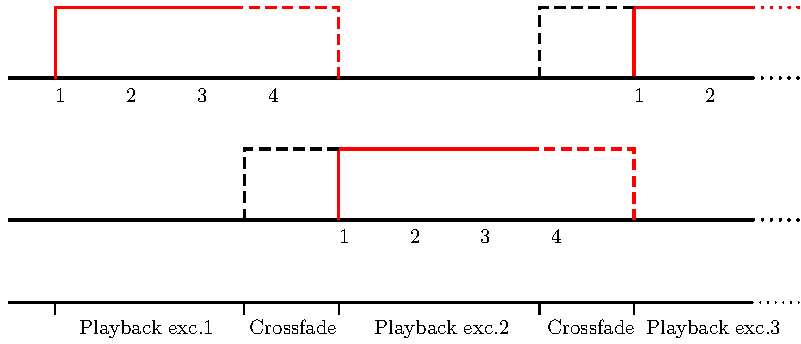
\includegraphics[scale=1]{Figures/crossfade.pdf}
    \rule{27em}{0.5pt}
  \caption[Crossfade handling]{Handling of crossfades. The red rectangles indicated the content of the excerpt, and dashed lines indicate crossfades. Note that the playback involves more than just the excerpts' content: we use the portion of audio before it during the fade-in to achieve a beat-level synchronization. The indices indicate the number of the beats inside the excerpts.}
  \label{fig:crossfade}
\end{center}
\end{figure}
\\The audio of the global pipeline is collected by the TCP sink, that is in charge of streaming this content over the TCP port 8070. This stream will be collected by the client application.


%%%%%%%%%%%%%%%%%%%%%%%%%%%%%%%%%%%%%%%%%%%%%%%%%%%%%%%%%%%%%%%%%%%%%%%%%%%%%%%%%%%%%%%%%%%%%%%%%%%%%%%%%%%%%%%%%%%%%%%%%%%%%%%%%%%%%%%%%%%%%%%%%%%%%%%%%%%%%%%%%%%%%%%%%%%%%%%%%%%%%%%%%%%%%%%%%%%%%%%%%%%%%%%
%%%%%%%%%%%%%%%%%%%%%%%%%%%%%%%%%%%%%%%%%%%%%%%%%%%%%%%%%%%%%%%%%%%%%%%%%%%%%%%%%%%%%%%%%%%%%%%%%%%%%%%%%%%%%%%%%%%%%%%%%%%%%%%%%%%%%%%%%%%%%%%%%%%%%%%%%%%%%%%%%%%%%%%%%%%%%%%%%%%%%%%%%%%%%%%%%%%%%%%%%%%%%%%
%%%%%%%%%%%%%%%%%%%%%%%%%%%%%%%%%%%%%%%%%%%%%%%%%%%%%%%%%%%%%%%%%%%%%%%%%%%%%%%%%%%%%%%%%%%%%%%%%%%%%%%%%%%%%%%%%%%%%%%%%%%%%%%%%%%%%%%%%%%%%%%%%%%%%%%%%%%%%%%%%%%%%%%%%%%%%%%%%%%%%%%%%%%%%%%%%%%%%%%%%%%%%%%
%%%%%%%%%%%%%%%%%%%%%%%%%%%%%%%%%%%%%%%%%%%%%%%%%%%%%%%%%%%%%%%%%%%%%%%%%%%%%%%%%%%%%%%%%%%%%%%%%%%%%%%%%%%%%%%%%%%%%%%%%%%%%%%%%%%%%%%%%%%%%%%%%%%%%%%%%%%%%%%%%%%%%%%%%%%%%%%%%%%%%%%%%%%%%%%%%%%%%%%%%%%%%%%

\section{The client application}
\label{sec:rtclient}
The client application consists of a web-application hosted by the Flask application running on the server. To access it, the client needs to connect to the address \texttt{http://server\_address:5000} on a browser. We entirely designed the graphical user interface of this application with the software \textit{Adobe Photoshop CS6\footnote{\url{http://www.adobe.com/products/photoshop.html}}}, with the intention of providing a ``metallic'' looking (that could resemble of the analogue synthesizers used in early Phonos records) coupled with the presence of elements (sliders and knob controllers) whose purpose could be easily understood by users. This interface is shown in Figure~\ref{fig:gui1}.

\begin{figure}[h]
\hskip -0.8cm
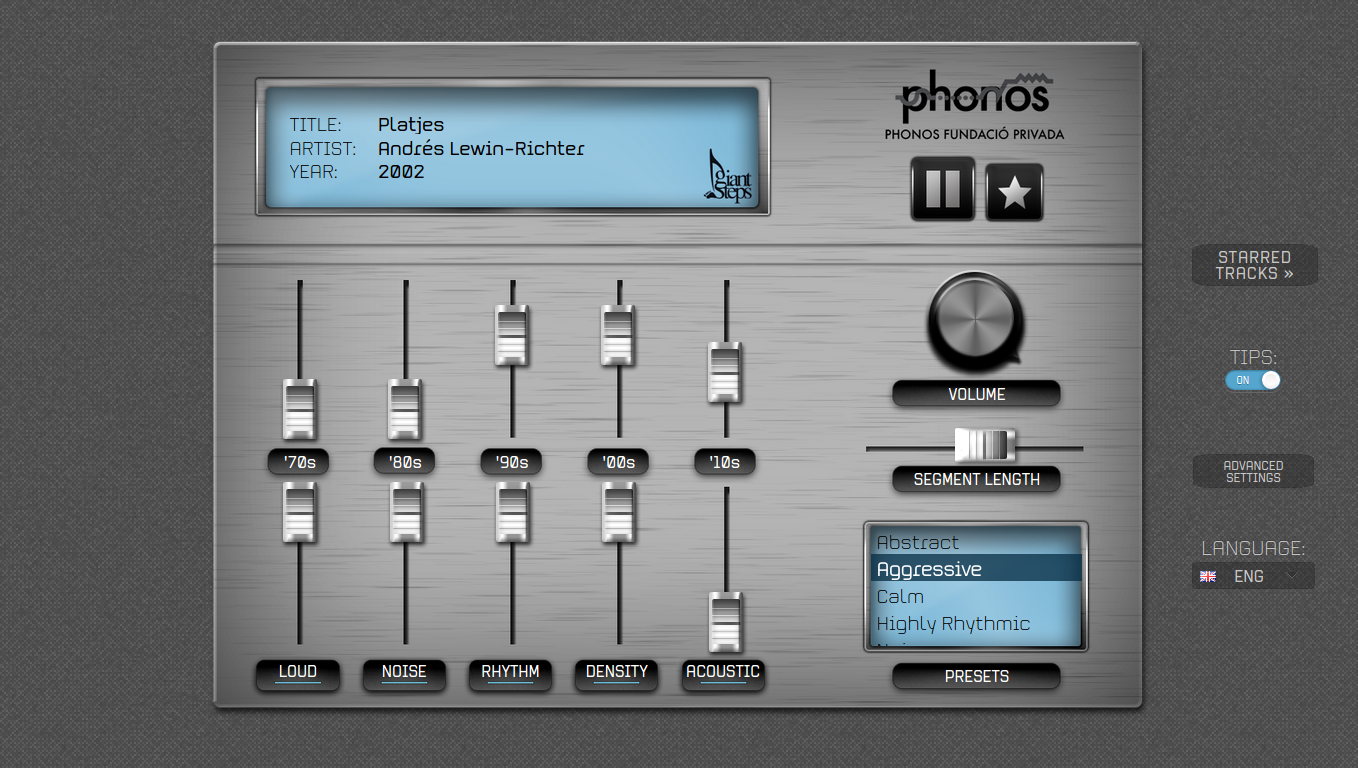
\includegraphics[scale=0.34]{Figures/gui1.png}
    \rule{27em}{0.5pt}
  \caption[Client application user interface]{Client application GUI.}
  \label{fig:gui1}

\end{figure}

This interface provides several ways for the user to control the music flow. Each time the user interacts with one of them, an HTTP post request is done from the client machine to the server, resulting in a change of the candidates for the playlist. \\
There are ten sliders: five of them are related to the year of release of the musical pieces, the other five are instead related to intrinsic characteristics of the music. In this way, the user has control both over the decade, and both over the type of music he wants to listen to. The motivation of this design choice is that we want to make the process of discovering music interactive while preserving ease of use. Furthermore, the suddivision of music into decades may be particularly useful in the use at the exhibition, since visitors could be particularly interested in hearing the differences between the works belonging to just a particular era over the entire 40 years life of Phonos. \\The five sliders for music features are:
\begin{itemize}
\item Loudness
\item Noisiness: related to the dissonance of the signal
\item Rhythm: higher values of the slider lead to excerpts with a high amount of onsets on high frequencies
\item Density: higher values of the slider lead to excerpts where many Barkbands have a considerable amount of energy
\item Acousticness: sets the ratio Acoustic/Electronic. Lower values of the slider mostly lead to purely electronic music.
\end{itemize}
The ranges of the internally managed sliders' values are dinamically generated during the computation of the FastMap: once the corresponding values for all the excerpts have been collected, these are sorted and we then pick the minimum, the maximum, and the first, second and third quartile for the values related to each descriptors. Therefore keeping the slider of the loudness at maximum will for instance lead to all the excerpts whose loudness value is between the third quartile and the maximum value of loudness of all excerpts. Step values for these five descriptors are calculated after the computation of the FastMap and kept in a separate JSON file. \\
The GUI additionally provides a set of presets for the values of these five sliders, a monitor for displaying information about the currently playing track, a slider for selecting the length of the audible segments (from 1 to 5 bars), and a knob for the volume (which controls the volume element of the global pipeline explained in Table~\ref{table:pipeline}). \\ By clicking on the button with a star on it, the user has the possibility of marking a track as favorite. The list of \textit{``starred tracks''} is accessible on the second page of the GUI (shown in Figure~\ref{fig:gui2}), together with the list of the five last played track. The motivation behind this choice is to give the user the chance to keep track of the songs he has been finding interesting. At the exhibition, visitors may be particularly interesting in looking for more information about a track they like. \\ 
Furthermore, this interface is offered in three different languages: English, Spanish and Catalan. This has been done to increase the usability of the software at the exhibition, taking into account possible cultural differences. \\
The interface fully supports touch screen environments and is based on HTML5, CSS3 and Javascript. Many features of the jQuery library for Javascript are also used. The range sliders are based on \textit{noUiSlider\footnote{\url{http://refreshless.com/nouislider/}}}, while the volume knob is based on \textit{jQuery Knob\footnote{\url{http://anthonyterrien.com/knob/}}}. The design of the graphical user interface has been directed toward the ease of use, for the visitors of the Museum may not be particularly confortable with the use of software or of tools related to music manipulation or playback. \\
Corcerning the reception of the audio streaming, many efforts have been done in order to achieve low-latency in the transmission of the multimedia content. Specifically, tries have involved the use of an icecast\footnote{\url{http://icecast.org/}} server or specific GStreamer units to try to implement low-latency audio streaming directly accessible from the html5 page. None of these tries have fully worked: latency was always registered around 5 seconds, probably due to browser's buffering techiques. This performance was clearly unacceptable. Thus we decided to exploit the functionalities provided by VideoLAN VLC\footnote{\url{http://www.videolan.org/vlc/index.html}}: specifically, we wrote a daemon for the interactive kiosk that launches a hidden instance of VLC as soon as it detects a stream on the TCP port 8070 (generated by the TCPSink of GStreamer). This istance of VLC is then in charge of capturing and playing this stream of multimedia content. The main advantages of this choice are:
\begin{itemize}
\item Good latency (around 500ms)
\item The user is completely unaware of this, for it is possible to start VLC in a daemon mode, thus without any sort of windows popping up. 
\end{itemize}
Generally, for real-time web application, the use of web protocols RTP (Real Time Protocol) and RTSP (Real Time Streaming Protocol) is suggested, as this usually allows low latencies in multimedia streaming. The use of these protocols for this application have not been taken into account, for their use requires to be integrated into Adobe Flash\footnote{\url{http://get.adobe.com/it/flashplayer/}} applications, which are generally discouraged as they introduce additional constraints and are usually not supported on touch devices. Furthermore, we had no experience with this particular programming language, and it could have not been feasible to develop the audio streaming in this language before the inauguration of the exhibition.

\begin{figure}[h]
\hskip -0.4cm
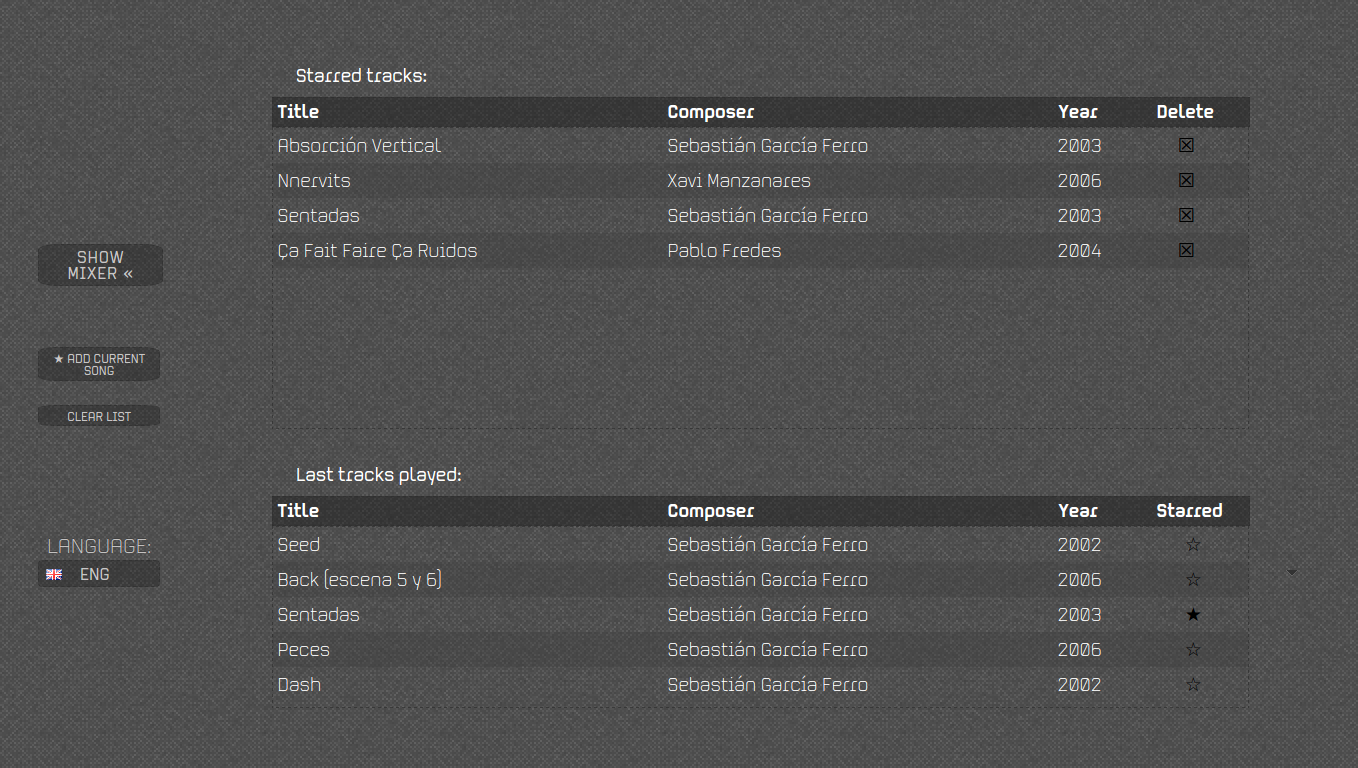
\includegraphics[scale=0.32]{Figures/gui2.png}
    \rule{27em}{0.5pt}
  \caption[The second page of the user interface]{The second page of the client application GUI, providing information about favorite and last played tracks.}
  \label{fig:gui2}
\end{figure}

The performance of this real-time system will be analyzed in the following chapter. 
\part{Results and Discussion}
\newpage
\thispagestyle{plain}
\mbox{}
\chapter{Results} 

\label{Chapter7} 

\lhead{Chapter 7. \emph{Results}}

\section{Performance}
Performance has been the main concern in the development of the system. As already seen in previous chapters, many efforts have been made in order to achieve a good responsiveness to user input in the real time application. We made the clear choice of preferring low times in the offline computation of descriptors (reported in Table~\ref{table:benchmarkoffline}) for this has helped us in achieving good response times in the real time application. The latter ones, in general, greatly vary with the use of the application. For instance, the user interaction with sliders has the effect of emptying the playlist queue (which will result in temporary shorter computational times, due to the use of the least precise but fastest music similarity computation algorithm in order to get some new element into the playlist as soon as possible), while choosing to use longer segments or not interacting with the sliders may increase the computational time (for the system realizes that it has more time available for computing music similarity and then uses the most accurate algorithm\footnote{We recall that the only difference between the two algorithms lies in the choice of the similarity function, as shown at the point 8 of Section~\ref{subsec:rtalgorithm}}). \\
For us, this instability of performance is not intended as a flaw: it could rather be seen as good flexibility of the system to many different computational situations.\\
We decided to collect data about computational times of the real time application for the choice of 1000 consecutive excerpts, with occasional interaction of the user. This is a reasonable analysis case, for it may be very similar to the real use of the system and also provides a good perspective on the computational times while using the most demanding algorithm of the system for computing music similarity. The results are shown for each main point of the procedure explained in Section~\ref{subsec:rtalgorithm}.

\begin{figure}[h]
\begin{center}
\includegraphics[scale=0.5]{Figures/figure_1.pgf}
    \rule{20em}{0.5pt}
  \caption[GStreamer]{GStreamer logo.}
  \label{fig:GStreamer}
\end{center}
\end{figure}


\section{Evaluation}
\section{Use at exhibition} 
\section{Results obtained by the study} 
\chapter{Conclusions and future work} 

\label{Chapter8} 

\lhead{Chapter 8. \emph{Conclusions and future work}}

We have developed a software that allows an easy, fast and enjoyable exploration of music collections. The main requirements for the system during the development have been:
\begin{itemize}
\item Responsiveness to real-time users' interaction
\item Ease of use
\item Enjoyability of musical flow
\end{itemize}
As shown in Chapter~\ref{Chapter7}, we achieved good results for each of these aspects. For doing this many efforts have been taken, especially in the design of the design: many ``little'' choices were taken in order to make the system as fast as possible. Most of the difficulties encountered were related to the generation of audio with Gstreamer (for which good documentation was generally lacking) and to the streaming of this audio content to the client machine with low latencies.  

\section{Contributions}
The main result achieved by the study was the exploitation of latest MIR findings for the development of a system that could easily be used by people not related to the research field and, more in general, not accustomed to the use of software. \\
This is a further proof that MIR technologies may be extremely useful in a wide range of applications, the most of which linked to common daily life situations. The software integrates not only different descriptors, but also different tools to extract them (Essentia and Echo Nest) in order to maximize the output, something that has rarely been done before.\\
Another contribution of this study lies in the integration of different researches into a single system: a study of of latest findings has been conducted in order to find what results have been achieved and could have been useful for our purposes. Despite being influenced by other solutions, ours constitutes an original way of solving the problem, for the algorithm we developed offer several new ideas; these are mainly due to the requirement of developing a low-latency system. Furthermore, the requirement of mixing together tracks (instead of just building a playlist of songs to be played one after another) has lead to the choice of implementing some personal musical knowledge in order to discard mixes that would have been perceived highly contrasting. This knowledge is especially related to the field of music composition and perception.\\

\section{Future work}
Despite having successfully reached its main goals, there is a lot of room for improving the system. \\
At first, the use of JSON files should be discarded in favour of much faster database tables, for instance PostgreSQL or MySQL. As seen in \ref{sec:performanceanalysis}, accessing and parsing JSON files is one of the slowest operations of the algorithm (almost 100 times longer than computing the symmetric Kullback-Leibler distance). Implementing a database should allow to use the more computationally intensive variant of the algorithm more frequently and to make the sampling less aggressive, therefore leading to generally better results. \\
The computation of music similarity could also be improved and use more sophisticated techniques, such as Fluctuation Patterns, that have shown very good results in similar systems \cite{pohle09}. \\
Furthermore, the development of a web application imposes several limitations (such as general low performances and high latency on audio streaming) that could easily be solved in a native mobile application for tablets or smartphones. \\
The source code for the application is entirely available at \url{https://github.com/giuband/Phonos-Music-Explorer}, so that many users can contribute in making it better.\\
Once the above cited aspects are refined, the development of the system could follow two different paths.
\begin{enumerate}
\item The system could be improved in its use for music discovery. For instance the user interface could implement some way of letting the user explore his current position inside the map of excerpts, in order to give a more clear idea about the music of the catalogue. New descriptors could be used and some of them could also be inherited from metadata or machine learning processes. 
\item The system could additionaly be integrated into a more creative environment for making music. It could be used for the automatic generation of recommendations while in the process of composing music. For instance, it could suggest the user of using a particular excerpt at some point of his composition to improve the quality of the work. It could also be used as the only source to compose music, providing the ability of automatically composing music made of excerpts while the user gives a direction to this flow, according to his creative intent. 
\end{enumerate}
The use suggested in 2. is particularly interesting, for such an application would perfectly fit the vision embraced by the GiantSteps project and provide a new system of producing music, making this amazing creative task accessible at anyone, indipendently from the skill. The process of making music could therefore overthrow its innate boundaries, leading to a world where the creation of art arises from the purest intent of contributing to the world cultural heritage, in spite of lack of limited technical knowledge, economic unavailability and physical impediments.
 

%----------------------------------------------------------------------------------------
%	THESIS CONTENT - APPENDICES
%----------------------------------------------------------------------------------------

\addtocontents{toc}{\vspace{2em}} % Add a gap in the Contents, for aesthetics

\appendix % Cue to tell LaTeX that the following 'chapters' are Appendices

% Include the appendices of the thesis as separate files from the Appendices folder
% Uncomment the lines as you write the Appendices

\chapter{List of Essentia descriptors} 

\label{AppendixA}

\lhead{Appendix A. \emph{List of Essentia descriptors}} 
As of November 2014, the features provided by Essentia 2.0.1 are:

\begin{center}
\begin{longtable}{ p{.15\textwidth} p{.25\textwidth} p{.45\textwidth} } 

\textbf{Category} & \textbf{Subcategory} & \textbf{Name} \\ \toprule
Low-level & Barkbands & Values\\ \cmidrule(r){3-3}
&  & Kurtosis \\ \cmidrule(r){3-3} 
&  & Skewness \\ \cmidrule(r){3-3}
&  & Spread \\ \cmidrule(r){2-3}
& Pitch & Value\\ \cmidrule(r){3-3}
& & Instantaneous confidence \\ \cmidrule(r){3-3}
& & Salience \\ \cmidrule(r){2-3}
& Spectral & Centroid \\ \cmidrule(r){3-3}
& & Complexity \\ \cmidrule(r){3-3}
& & Crest \\ \cmidrule(r){3-3}
& & Decrease \\ \cmidrule(r){3-3}
& & Energy \\ \cmidrule(r){3-3}
& & Energyband high \\ \cmidrule(r){3-3}
& & Energyband low \\ \cmidrule(r){3-3}
& & Energyband middle high \\ \cmidrule(r){3-3}
& & Energyband middle low \\ \cmidrule(r){3-3}
& & Flatness db \\ \cmidrule(r){3-3}
& & Flux \\ \cmidrule(r){3-3}
& & Kurtosis \\ \cmidrule(r){3-3}
& & Rms \\ \cmidrule(r){3-3}
& & Rolloff \\ \cmidrule(r){3-3}
& & Skewness \\ \cmidrule(r){3-3}
& & Spread \\ \cmidrule(r){3-3}
& & Strongpeak \\ \cmidrule(r){2-3}
& Other & Average loudness \\ \cmidrule(r){3-3}
& & Dissonance \\ \cmidrule(r){3-3}
& & Hfc \\ \cmidrule(r){3-3}
& & Mfcc \\ \cmidrule(r){3-3}
& & Sccoeffs \\ \cmidrule(r){3-3}
& & Scvalleys \\ \cmidrule(r){3-3}
& & Silence rate 30dB \\ \cmidrule(r){3-3}
& & Silence rate 30dB \\ \cmidrule(r){3-3}
& & Silence rate 60dB \\ \cmidrule(r){3-3}
& & Zerocrossingrate \\ \midrule
Rhythm & Beats & Position \\ \cmidrule(r){3-3}
& & Loudness \\ \cmidrule(r){3-3}
& & Loudness band ratio \\ \cmidrule(r){2-3}
& BPM & Value \\ \cmidrule(r){3-3}
& & Estimates \\ \cmidrule(r){3-3}
& & Intervals \\ \cmidrule(r){2-3}
& First peak & BPM \\ \cmidrule(r){3-3}
& & Spread \\ \cmidrule(r){3-3}
& & Weight \\ \cmidrule(r){2-3}
& Onset & Onset Rate \\ \cmidrule(r){3-3}
& & Onset Times \\ \cmidrule(r){2-3}
& Second peak & BPM \\ \cmidrule(r){3-3}
& & Spread \\ \cmidrule(r){3-3}
& & Weight \\ \midrule
Sfx & Pitch & After max to before max energy ratio \\ \cmidrule(r){3-3}
& & Centroid \\ \cmidrule(r){3-3}
& & Max to total \\ \cmidrule(r){3-3}
& & Min to total \\ \cmidrule(r){2-3}
& Other & Inharmonicity \\ \cmidrule(r){3-3}
& & Oddtoeven harmonic energy ratio \\ \cmidrule(r){3-3}
& & Tristimulus \\ \midrule
Tonal & Chords & Changes rate \\ \cmidrule(r){3-3}
& & Histogram \\ \cmidrule(r){3-3}
& & Key \\ \cmidrule(r){3-3}
& & Number rate \\ \cmidrule(r){3-3}
& & Progression \\ \cmidrule(r){3-3}
& & Scale \\ \cmidrule(r){3-3}
& & Strength \\ \cmidrule(r){3-3}
& & HPCP \\ \cmidrule(r){2-3}
& Key & Value \\ \cmidrule(r){3-3}
& & Scale \\ \cmidrule(r){3-3}
& & Strength \\ \cmidrule(r){3-3}
& & Thpcp \\ \cmidrule(r){2-3}
& Tuning & Diatonic strength \\ \cmidrule(r){3-3}
& & Equal tempered deviation \\ \cmidrule(r){3-3}
& & Frequency \\ \cmidrule(r){3-3}
& & Nontempered energy ratio \\ \bottomrule

\caption[List of features computable with Essentia]{List of features computable with Essentia.}
\label{table:essentiaFeatures}
\end{longtable}
\end{center}
\chapter{List of Echonest Features} % Main appendix title

\label{AppendixB} % For referencing this appendix elsewhere, use \ref{AppendixA}

\lhead{Appendix B. \emph{List of Echonest Features}} % This is for the header on each page - perhaps a shortened title

Write your Appendix content here.
\chapter{Phonos: list of songs} 

\label{AppendixC} 

\lhead{Appendix C. \emph{Phonos: list of songs}} 

The musical pieces to be used during the \textit{``Phonos, 40 anys de música electrònica a Barcelona''} exhibition at Museu de la Musica (L'Auditori, Carrer de Lepant, 150, 08013 Barcelona) are: 

\begin{center}
\begin{longtable}{ p{.35\textwidth}  p{.57\textwidth}  p{.08\textwidth} } 
\textbf{Artist} & \textbf{Title} & \textbf{Year} \\ \toprule
Alain Perón & De Dos Para Uno & 1996 \\ \cmidrule(r){2-3}
& Los Edictos & 1998 \\ \midrule 
Albert Llanas & Nexus & 1999 \\ \cmidrule (r){2-3}
& Formants & 2004 \\ \midrule 
Alejandro Martínez & Monoleg & N.A. \\ \cmidrule (r){2-3}
& Helesponto & 1982 \\ \cmidrule (r){2-3}
& Tazir & 1984 \\ \cmidrule (r){2-3}
& Crisálida & 1987 \\ \cmidrule (r){2-3} 
& Machina animata & 1987 \\ \cmidrule (r){2-3} 
& Canción de Otoño & 1989 \\ \cmidrule (r){2-3} 
& Homenaje L.Nono & 1990 \\ \cmidrule (r){2-3} 
& Música Palimpesto & 1991 \\ \cmidrule (r){2-3} 
& Vaciando el hueco & 1996 \\ \midrule  
Alex Arteaga & Témenos & 2006 \\ \midrule 
Alex Geell & Panales & 2010 \\ \midrule 
Alex Sanjurjo & Fluir & 2003 \\ \midrule \midrule 
Alexandra Gardner & Ayehli & 2002 \\ \cmidrule (r){2-3}  
& Snapdragon & 2002 \\ \cmidrule (r){2-3}   
& New Skin & 2003 \\ \cmidrule (r){2-3}   
& Onice & 2003 \\ \cmidrule (r){2-3}   
& Luminoso & 2004 \\ \cmidrule (r){2-3}   
& Tourmaline & 2004 \\ \midrule 
Alexandre Marino & Apparatus, Experimentalis & 2008 \\ \cmidrule (r){2-3}
& Apparatus, Musical & 2008 \\ \midrule 
Andrés Lewin-Richter & Joc - Eventos & 1976 \\ \cmidrule (r){2-3} 
& Joc - Fondo & 1976 \\ \cmidrule (r){2-3} 
& Acción 2 - 1 & 1978 \\ \cmidrule (r){2-3} 
& Acción 2 - 2 & 1978 \\ \cmidrule (r){2-3} 
& Acción 2 - 3 & 1978 \\ \cmidrule (r){2-3} 
& Acción 2 - 4 & 1978 \\ \cmidrule (r){2-3} 
& Giravolt & 1978 \\ \cmidrule (r){2-3} 
& El Paraiso & 1979 \\ \cmidrule (r){2-3} 
& El Viento I - 1 & 1979 \\ \cmidrule (r){2-3} 
& El Viento I - 2 & 1979 \\ \cmidrule (r){2-3} 
& El Viento I - 3 & 1979 \\ \cmidrule (r){2-3} 
& El Viento II & 1979 \\ \cmidrule (r){2-3} 
& Reacciones I II & 1979 \\ \cmidrule (r){2-3} 
& Secuencia IV & 1979 \\ \cmidrule (r){2-3} 
& Baschetiada & 1980 \\ \cmidrule (r){2-3} 
& El Viento III & 1980 \\ \cmidrule (r){2-3} 
& El Viento IV & 1980 \\ \cmidrule (r){2-3} 
& Reacciones III & 1980 \\ \cmidrule (r){2-3} 
& Wagler Walricci & 1981 \\ \cmidrule (r){2-3} 
& Actualidad discográfica & 1982 \\ \cmidrule (r){2-3} 
& Sones & 1982 \\ \cmidrule (r){2-3} 
& 6 Songs & 1983 \\ \cmidrule (r){2-3} 
& Quorum & 1983 \\ \cmidrule (r){2-3} 
& Secuencia V & 1983 \\ \cmidrule (r){2-3} 
& Secuencia VI & 1983 \\ \cmidrule (r){2-3} 
& Tinell & 1983 \\ \cmidrule (r){2-3} 
& Cogida & 1984 \\ \cmidrule (r){2-3} 
& In memoriam Manuel Valls & 1984 \\ \cmidrule (r){2-3} 
& Isaac el Cec & 1984 \\ \cmidrule (r){2-3} 
& Juegos & 1985 \\ \cmidrule (r){2-3} 
& Musica electroacústica & 1985 \\ \cmidrule (r){2-3} 
& Solars Vortices & 1985 \\ \cmidrule (r){2-3} 
& Desfigurat & 1986 \\ \cmidrule (r){2-3} 
& Diálogos & 1987 \\ \cmidrule (r){2-3} 
& Secuencia VII & 1987 \\ \cmidrule (r){2-3} 
& Homenaje a Zinovieff & 1988 \\ \cmidrule (r){2-3} 
& Secuencia VIII & 1988 \\ \cmidrule (r){2-3} 
& Verra la Morte & 1988 \\ \cmidrule (r){2-3} 
& Verra la Morte 1 & 1988 \\ \cmidrule (r){2-3} 
& Verra la Morte 2 & 1988 \\ \cmidrule (r){2-3} 
& Verra la Morte 3 & 1988 \\ \cmidrule (r){2-3} 
& Verra la Morte 4 & 1988 \\ \cmidrule (r){2-3} 
& Verra la Morte 5 & 1988 \\ \cmidrule (r){2-3} 
& Verra la Morte 6 & 1988 \\ \cmidrule (r){2-3} 
& Verra la Morte 7 & 1988 \\ \cmidrule (r){2-3} 
& Verra la Morte 8 & 1988 \\ \cmidrule (r){2-3} 
& 99 Golpes & 1989 \\ \cmidrule (r){2-3} 
& Ben avra questa donna cor di ghiacio & 1989 \\ \cmidrule (r){2-3} 
& Secuencia IX & 1989 \\ \cmidrule (r){2-3} 
& Strings & 1989 \\ \cmidrule (r){2-3} 
& Brossiana & 1990 \\ \cmidrule (r){2-3} 
& Donne Fiori & 1990 \\ \cmidrule (r){2-3} 
& Fragmento (a Nono) & 1990 \\ \cmidrule (r){2-3} 
& Frullato & 1990 \\ \cmidrule (r){2-3} 
& Ludus Basiliensis & 1991 \\ \cmidrule (r){2-3} 
& Reacciones IV & 1991 \\ \cmidrule (r){2-3} 
& Secuencia X & 1991 \\ \cmidrule (r){2-3} 
& Radio 2 & 1996 \\ \cmidrule (r){2-3} 
& Sarangi & 1999 \\ \cmidrule (r){2-3} 
& Configuraciones & 2000 \\ \cmidrule (r){2-3} 
& Constelaciones & 2000 \\ \cmidrule (r){2-3} 
& Figuras & 2000 \\ \cmidrule (r){2-3} 
& Resonancias & 2000 \\ \cmidrule (r){2-3} 
& Secuencia XI & 2001 \\ \cmidrule (r){2-3} 
& Secuencia XII & 2001 \\ \cmidrule (r){2-3} 
& Dreams & 2002 \\ \cmidrule (r){2-3} 
& Ludus Allavarium & 2002 \\ \cmidrule (r){2-3} 
& Platjes & 2002 \\ \cmidrule (r){2-3} 
& Secuencia XIII & 2002 \\ \cmidrule (r){2-3} 
& Signals & 2002 \\ \cmidrule (r){2-3} 
& Viso di Primavera & 2002 \\ \cmidrule (r){2-3} 
& Fantasia & 2003 \\ \cmidrule (r){2-3} 
& Juego de Acordeón & 2003 \\ \cmidrule (r){2-3} 
& Meisoh No Ne & 2003 \\ \cmidrule (r){2-3} 
& Melodias & 2003 \\ \cmidrule (r){2-3} 
& Metálica & 2003 \\ \cmidrule (r){2-3} 
& Omaggio a Berio: sequenza per tuba & 2003 \\ \cmidrule (r){2-3} 
& Secuencia XIV & 2003 \\ \cmidrule (r){2-3} 
& Essay on Trombone & 2004 \\ \cmidrule (r){2-3} 
& Fragments & 2004 \\ \cmidrule (r){2-3} 
& Secuencia  XV & 2004 \\ \cmidrule (r){2-3} 
& Arssonxx.rne & 2005 \\ \cmidrule (r){2-3} 
& Fluxus es zen? & 2005 \\ \cmidrule (r){2-3} 
& Interacciones & 2006 \\ \cmidrule (r){2-3} 
& On "Freesound" Water & 2006 \\ \cmidrule (r){2-3} 
& Secuencia XVI & 2006 \\ \cmidrule (r){2-3} 
& For Harry & 2007 \\ \cmidrule (r){2-3} 
& Retales & 2007 \\ \cmidrule (r){2-3} 
& Sombras & 2007 \\ \cmidrule (r){2-3} 
& Soplos & 2007 \\ \cmidrule (r){2-3} 
& Sospiri & 2007 \\ \cmidrule (r){2-3} 
& Friendship Quartet & 2008 \\ \cmidrule (r){2-3} 
& Homenaje a Pierre Schaeffer & 2008 \\ \cmidrule (r){2-3} 
& Makeup & 2008 \\ \cmidrule (r){2-3} 
& Schaeffer granulado & 2008 \\ \cmidrule (r){2-3} 
& Aire & 2009 \\ \cmidrule (r){2-3} 
& Génesis & 2009 \\ \cmidrule (r){2-3} 
& Homenaje a Varese & 2009 \\ \cmidrule (r){2-3} 
& Memento & 2009 \\ \cmidrule (r){2-3} 
& Paseo BCN & 2009 \\ \cmidrule (r){2-3} 
& Sancta Maria & 2009 \\ \cmidrule (r){2-3} 
& Slapring & 2009 \\ \cmidrule (r){2-3} 
& Spring & 2009 \\ \cmidrule (r){2-3} 
& Imagenes & 2010 \\ \cmidrule (r){2-3} 
& Secuencia XVIII Fagot & 2010 \\ \cmidrule (r){2-3} 
& Multifonia & 2011 \\ \cmidrule (r){2-3} 
& Campanas para una celebracion & 2012 \\ \cmidrule (r){2-3} 
& Multifonia III & 2012 \\ \cmidrule (r){2-3} 
& Secuencia XIX & 2014 \\ \midrule
Anna Bofill & Espai Sonor & N.A. \\ \cmidrule (r){2-3}
& Trio para Violin y Cinta & N.A. \\ \midrule 
Ariadna Alsina & Sinapsis & 2006 \\ \cmidrule (r){2-3}
& Reconstrucció & 2011 \\ \cmidrule (r){2-3}
& Vels Vitris & 2012 \\ \midrule 
Ariadna Alsina \& David Salleras & Contramarea & 2009 \\ \midrule 
Arturo Moya & La Música Que Había en Mis Objetos & 1996 \\ \cmidrule (r){2-3} 
& Estampas de Caza 1 & 2000 \\ \cmidrule (r){2-3} 
& Estampas de Caza 2 & 2000 \\ \cmidrule (r){2-3} 
& Estampas de Caza 4 & 2000 \\ \cmidrule (r){2-3} 
& Estampas de Caza 5 & 2000 \\ \midrule 
Arturo Palaudaria & Estate quieto Voltaire & N.A. \\ \cmidrule (r){2-3} 
& Adolescencia y Estrella & 1980 \\ \cmidrule (r){2-3} 
& Escudellers & 1981 \\ \cmidrule (r){2-3} 
& Piamo & 1984 \\ \cmidrule (r){2-3} 
& Toda la Memoria de un Hombre & 1987 \\ \cmidrule (r){2-3} 
& El Destino de las Cosas & 1988 \\ \cmidrule (r){2-3} 
& La Luz de los Sueños & 1989 \\ \cmidrule (r){2-3} 
& Boule de Feu & 1990 \\ \cmidrule (r){2-3} 
& Paréntesis militar & 1990 \\ \cmidrule (r){2-3} 
& El Juicio Estético Universal & 1991 \\ \cmidrule (r){2-3} 
& Moverse en el Tiempo & 1997 \\ \midrule 
Aurelio Edler-Copes & Women in Process & 2013 \\ \midrule 
Cadavers & Exquisits & 2003 \\ \midrule 
Carlos Lupprián & Latido & 1995 \\ \cmidrule (r){2-3} 
& Agugagá & 1996 \\ \cmidrule (r){2-3} 
& Naturaleza Muerta & 1997 \\ \midrule 
Claudio Nervi & Improvisación con Oratio Trio & 2010 \\ \midrule 
Claudio Zulian & Valent La Notte & N.A. \\ \cmidrule (r){2-3} 
& El Libro de los Excesos & 1983 \\ \cmidrule (r){2-3} 
& San Claudio Vive Solo & 1985 \\ \cmidrule (r){2-3} 
& Sexo y Politica & 1987 \\ \cmidrule (r){2-3} 
& I Quattro Continenti & 1989 \\ \cmidrule (r){2-3} 
& Por de Ser Set & 1989 \\ \cmidrule (r){2-3} 
& Sueños Ecléctricos & 1989 \\ \cmidrule (r){2-3} 
& Variazione Angelica & 1990 \\ \cmidrule (r){2-3} 
& 2 Escenas de Macbeth - 1 & 1991 \\ \cmidrule (r){2-3} 
& 2 Escenas de Macbeth - 2 Ruidos & 1991 \\ \midrule 
Concha Trallero & Armonias 1 & 1980 \\ \cmidrule (r){2-3} 
& Armonias 2 & 1980 \\ \cmidrule (r){2-3} 
& Armonías Sonoras 1 & 1980 \\ \cmidrule (r){2-3} 
& Armonías Sonoras 2 & 1980 \\ \midrule 
Cristián López & Leftraru, Viajero Ensoñado - El Río de la Vida & 2005 \\ \cmidrule (r){2-3} 
& Leftraru, Viajero Ensoñado - Espírutu Azul & 2005 \\ \cmidrule (r){2-3} 
& Leftraru, Viajero Ensoñado - Interludio & 2005 \\ \cmidrule (r){2-3} 
& Leftraru, Viajero Ensoñado - Piedra Solitaria & 2005 \\ \cmidrule (r){2-3} 
& Leftraru, Viajero Ensoñado - Relámpago Azul & 2005 \\ \midrule 
Relief II & Cristián Morales-Ossio & 2001 \\ \midrule 
Daniel Domínguez Teruel & TRTPS & 2010 \\ \cmidrule (r){2-3} 
& SKTHN & 2012 \\ \cmidrule (r){2-3} 
& Study I & 2013 \\ \cmidrule (r){2-3} 
& Study II & 2013 \\ \cmidrule (r){2-3} 
& Study V & 2013 \\ \midrule
Daniel Rios Aranda & Say It & 1987 \\ \cmidrule (r){2-3} 
& Erial & 1990 \\ \midrule 
Danilo Vidotti & Sueños & 2008 \\ \midrule 
Danio Catanuto & Psicofonias Urbanas 1 & 2010 \\ \cmidrule (r){2-3} 
& Psicofonias Urbanas 2 & 2010 \\ \midrule 
Darío Cortés & Formantes & 1998 \\ \midrule 
David Dalmazzo & Pulsajes & 2010 \\ \midrule 
David Padros & Confluencies & 1985 \\ \midrule 
Diego Dall'Osto & Caosmofonia & 1998 \\ \midrule 
Doénado, el Ur & Kinoko Tabí & 1988 \\ \cmidrule (r){2-3} 
& Pedicoj en la Arena del Pamir & 1989 \\ \cmidrule (r){2-3} 
& Zalody & 1990 \\ \cmidrule (r){2-3} 
& Yñé do zalod & 1991 \\ \cmidrule (r){2-3} 
& A Sensu Contrario & 1992 \\ \cmidrule (r){2-3} 
& Blordt Prelar & 1992 \\ \cmidrule (r){2-3} 
& Kzadzak & 1994 \\ \midrule 
Edgar Barroso & Tu Mateix & 2004 \\ \cmidrule (r){2-3} 
& Dux & 2005 \\ \cmidrule (r){2-3} 
& Tau & 2005 \\ \cmidrule (r){2-3} 
& Tu Soplo Que Transporta & 2005 \\ \cmidrule (r){2-3} 
& IOD & 2006 \\ \cmidrule (r){2-3} 
& CYT & 2007 \\ \midrule 
Edson Zampronha & Mármore & 2001 \\ \cmidrule (r){2-3} 
& Mármore 1 & 2001 \\ \cmidrule (r){2-3} 
& Mármore 2 & 2001 \\ \cmidrule (r){2-3} 
& Mármore 3 & 2001 \\ \midrule 
Eduard Resina & Read my LISP & 1991 \\ \cmidrule (r){2-3} 
& L'Esquizofrènia Dels Sons & 1993 \\ \cmidrule (r){2-3} 
& Aca Amaron & 2001 \\ \cmidrule (r){2-3} 
& L'Anna-crusa & 2002 \\ \midrule 
Eduardo Polonio & Espai Sonor & 1976 \\ \midrule 
Eduardo Reck Miranda & Requiem per una Veu Perduda & 1997 \\ \midrule 
Elsa Justel & Midi de Sable & 2000 \\ \midrule 
Enrique Marín & Elementos Constantes, Hechos Variables & 2002 \\ \cmidrule (r){2-3} 
& Transiciones de Fase & 2007 \\ \midrule \\ \midrule  
Ensamble Crumble y ReacTable & Untitled 1 & 2006 \\ \cmidrule (r){2-3} 
& Untitled 2 & 2006 \\ \cmidrule (r){2-3} 
& Untitled 3 & 2006 \\ \cmidrule (r){2-3} 
& Untitled 4 & 2006 \\ \cmidrule (r){2-3} 
& Untitled 5 & 2006 \\ \cmidrule (r){2-3} 
& Untitled 6 & 2006 \\ \cmidrule (r){2-3} 
& Untitled 7 & 2006 \\ \midrule 
FMOL Trio & Untitled 1 & 2001 \\ \cmidrule (r){2-3} 
& Untitled 2 & 2001 \\ \cmidrule (r){2-3} 
& Untitled 3 & 2001 \\ \midrule 
Felipe Pérez Santiago & CampoSanto & 2004 \\ \cmidrule (r){2-3} 
& Encandilado & 2007 \\ \cmidrule (r){2-3} 
& Hunger FM & 2009 \\ \cmidrule (r){2-3} 
& Hurt & 2009 \\ \cmidrule (r){2-3} 
& Ishmael & 2009 \\ \cmidrule (r){2-3} 
& Miuk & 2009 \\ \cmidrule (r){2-3} 
& Post War & 2009 \\ \cmidrule (r){2-3} 
& Tacto & 2009 \\ \cmidrule (r){2-3} 
& War-Post War & 2009 \\ \cmidrule (r){2-3} 
& Pronto Desapareceremos & 2012 \\ \midrule 
Fernando Jobke & Ecos 1 & 2008 \\ \cmidrule (r){2-3} 
& Ecos 2 & 2008 \\ \cmidrule (r){2-3} 
& Ecos 3 & 2008 \\ \cmidrule (r){2-3} 
& Ecos 4 & 2008 \\ \cmidrule (r){2-3} 
& Ecos 5 & 2008 \\ \cmidrule (r){2-3} 
& Ecos 6 & 2008 \\ \midrule 
Félix Luque \& Ricardo Gadea & Cuerpos Sensibles & 2005 \\ \midrule \\ \\ \midrule  
Félix Luque \& Thomas Charveriat & The Machine Manifesto & 2004 \\ \midrule 
Gabriel Brncic & Batucada Amenazante & 1970 \\ \cmidrule (r){2-3} 
& El Túnel (a Ernesto Sabato) & 1970 \\ \cmidrule (r){2-3} 
& Agua 1 & 1971 \\ \cmidrule (r){2-3} 
& Agua 2 & 1971 \\ \cmidrule (r){2-3} 
& Agua 3 & 1971 \\ \cmidrule (r){2-3} 
& Cielo & 1980 \\ \cmidrule (r){2-3} 
& Destierro & 1980 \\ \cmidrule (r){2-3} 
& Chile Fértil Provincia & 1983 \\ \cmidrule (r){2-3} 
& Concert Gothique & 1985 \\ \cmidrule (r){2-3} 
& Operas Rotas & 1985 \\ \cmidrule (r){2-3} 
& Clarinen Tres & 1986 \\ \cmidrule (r){2-3} 
& Clarinen Tres & 1986 \\ \cmidrule (r){2-3} 
& Desêtre a Oscar Masotta & 1986 \\ \cmidrule (r){2-3} 
& Triunfo Para las Madres & 1986 \\ \cmidrule (r){2-3} 
& Aria y Pasacalle & 1987 \\ \cmidrule (r){2-3} 
& Ese Mar & 1987 \\ \cmidrule (r){2-3} 
& Música de cámara & 1987 \\ \cmidrule (r){2-3} 
& Historia de Dos Ciudades & 1988 \\ \cmidrule (r){2-3} 
& Alegrias & 1989 \\ \cmidrule (r){2-3} 
& Composición de 1989 a Eduardo Polonio & 1989 \\ \cmidrule (r){2-3} 
& Dulcian Concert & 1989 \\ \cmidrule (r){2-3} 
& ariaciones sobre Sonatas e Interludios & 1989 \\ \cmidrule (r){2-3} 
& Adagio-Scherzo & 1990 \\ \cmidrule (r){2-3} 
& Vade Retro a Luigi Nono & 1990 \\ \cmidrule (r){2-3} 
& Dos Esbozos Para Antiguos Instrumentos Electrónicos & 1994 \\ \cmidrule (r){2-3} 
& ...Que No Desorganitza Cap Murmuri & 1995 \\ \cmidrule (r){2-3} 
& Constanza & 1996 \\ \cmidrule (r){2-3} 
& Claro-Oscuro & 1998 \\ \cmidrule (r){2-3} 
& Meng & 1998 \\ \cmidrule (r){2-3} 
& Clarinet Concert & 1999 \\ \cmidrule (r){2-3} 
& Coreutica & 1999 \\ \cmidrule (r){2-3} 
& Ergon-Rondeau & 2000 \\ \cmidrule (r){2-3} 
& A Joan Miró & 2001 \\ \cmidrule (r){2-3} 
& Alto-Concert II & 2001 \\ \cmidrule (r){2-3} 
& Bass clarinet-Concert for Harry Sparnaay & 2003 \\ \cmidrule (r){2-3} 
& Son(ru)idos I & 2003 \\ \cmidrule (r){2-3} 
& Son(ru)idos II & 2003 \\ \cmidrule (r){2-3} 
& La Casa del Viento 1 & 2006 \\ \cmidrule (r){2-3} 
& La Casa del Viento 2 & 2006 \\ \midrule 
Gaspar Lukacs Esguep & Pregoneros de Barcelona & 2002 \\ \midrule 
Germán Brull Moreno & Sin título & 2004 \\ \cmidrule (r){2-3} 
& Sin título & 2004 \\ \midrule 
Graciela Muñoz Farida & Arboleda & 2011 \\ \cmidrule (r){2-3} 
& Fragmentos de un Arbol & 2011 \\ \cmidrule (r){2-3} 
& Lo Que No Das Te Lo Quitas & 2011 \\ \cmidrule (r){2-3} 
& Viento Sur & 2011 \\ \midrule 
Graeme Truslove & Piece for Guitar and Tape & 2001 \\ \midrule 
Graham Coleman & Improvisation & 2007 \\ \cmidrule (r){2-3} 
& Improvisation & 2007 \\ \midrule 
Guillermo Eisner & Guitarrísticamente & 2007 \\ \midrule 
Igor Bimsbergen & Duo Para Siete & 1996 \\ \cmidrule (r){2-3} 
& Luis y Marylin & 1998 \\ \midrule 
Ismael Sanoja \& Kai Kraatz & Free What & 2006 \\ \cmidrule (r){2-3} 
& Free What 1 & 2006 \\ \cmidrule (r){2-3} 
& Free What 2 & 2006 \\ \cmidrule (r){2-3} 
& Free What 3 & 2006 \\ \cmidrule (r){2-3} 
& Free What 4 & 2006 \\ \cmidrule (r){2-3} 
& Free What 5 & 2006 \\ \cmidrule (r){2-3} 
& Free What 6 & 2006 \\ \cmidrule (r){2-3} 
& Free What 7 & 2006 \\ \cmidrule (r){2-3} 
& Free What 8 & 2006 \\ \midrule 
Jan Schacher & Traumtäntze & 2000 \\ \midrule 
Javier Navarrete & Preludios & 1976 \\ \midrule 
Jelena Vico & Almogavers & 2008 \\ \cmidrule (r){2-3} 
& Brithm & 2008 \\ \cmidrule (r){2-3} 
& Mrzbw & 2008 \\ \cmidrule (r){2-3} 
& Pangea & 2008 \\ \cmidrule (r){2-3} 
& Zeno & 2008 \\ \cmidrule (r){2-3} 
& Zitar & 2008 \\ \midrule 
Jep Nuix & Gallinària & 1980 \\ \cmidrule (r){2-3} 
& Doble Peça de Lletres i Sons & 1981 \\ \cmidrule (r){2-3} 
& Tres Canons de Noces & 1981 \\ \cmidrule (r){2-3} 
& Ad Valorem & 1984 \\ \cmidrule (r){2-3} 
& Halterofilia 1 & 1984 \\ \cmidrule (r){2-3} 
& Serenata Nocturna & 1985 \\ \cmidrule (r){2-3} 
& L'Inizio & 1986 \\ \cmidrule (r){2-3} 
& Dit a Dit, Pas a Pas & 1988 \\ \cmidrule (r){2-3} 
& Asirara & 1989 \\ \cmidrule (r){2-3} 
& Monoleg & 1989 \\ \cmidrule (r){2-3} 
& Trialeg & 1989 \\ \cmidrule (r){2-3} 
& His Master's Voice & 1990 \\ \cmidrule (r){2-3} 
& Improvisació per a tubs & 1990 \\ \cmidrule (r){2-3} 
& Pensant en Nono & 1990 \\ \cmidrule (r){2-3} 
& Percuflu & 1990 \\ \cmidrule (r){2-3} 
& Atentament & 1992 \\ \cmidrule (r){2-3} 
& Stack & 1995 \\ \midrule 
Joan Bagés i Rubí & Intersections-BouleWav 2.0 & 2006 \\ \midrule 
Joan Josep Ordinas \& Claudio Zulian & Al Tranquilodromo & 1981 \\ \midrule 
Joan Sanmarti & Passadis & 2001 \\ \cmidrule (r){2-3} 
& Reflexos Improvisacxiones Asistidas por Ordenador & 1997 \\ \cmidrule (r){2-3} 
& Xtrapolució 4 & 1998 \\ \midrule 
Jordi Rossinyol & Ricercare a 5 & 1986 \\ \cmidrule (r){2-3} 
& Objectes Trobats a la Platja & 1987 \\ \cmidrule (r){2-3} 
& Ocellots & 1988 \\ \cmidrule (r){2-3} 
& Mòbils Inquiets i Altres Equivocs & 1989 \\ \cmidrule (r){2-3} 
& Prosper Laberint Intermitent & 1990 \\ \cmidrule (r){2-3} 
& Variaciones guit & 1990 \\ \cmidrule (r){2-3} 
& Concert Mestis & 1997 \\ \cmidrule (r){2-3} 
& Ecliptic & 2004 \\ \midrule 
Jorge Sad & El Doble Bandoneón & 1998 \\ \cmidrule (r){2-3} 
& La Ida Hacia Abajo de la Tierra de la Tarde & 1999 \\ \midrule 
Josep Maria Guix & Landscape & 2010 \\ \cmidrule (r){2-3} 
& Landscape & 2010 \\ \cmidrule (r){2-3} 
& Landscape & 2010 \\ \midrule 
Josep Maria Mestres Quadreny & Oxo & 1963 \\ \cmidrule (r){2-3} 
& Peça per a Serra Mecanica & 1963 \\ \cmidrule (r){2-3} 
& Homenaje a Galileo & 1965 \\ \cmidrule (r){2-3} 
& Trois Cánones en Hommage à Galilea & 1968 \\ \cmidrule (r){2-3} 
& Aronada & 1972 \\ \cmidrule (r){2-3} 
& El Teler de Teresa Codina & 1973 \\ \cmidrule (r){2-3} 
& Song for Jane Manning & 1973 \\ \cmidrule (r){2-3} 
& Espai Sonor & 1976 \\ \cmidrule (r){2-3} 
& Espai Sonor & 1976 \\ \cmidrule (r){2-3} 
& Quina & 1979 \\ \cmidrule (r){2-3} 
& Cánones a Galileo & 1989 \\ \midrule 
José Manuel Berenguer & El Pensamiento Que Se Trabaja Hacia la Luz & N.A. \\ \cmidrule (r){2-3} 
& Spira & N.A. \\ \cmidrule (r){2-3} 
& Montardo & 1983 \\ \cmidrule (r){2-3} 
& A Florats & 1984 \\ \cmidrule (r){2-3} 
& La Logica de la Sorpresa & 1984 \\ \cmidrule (r){2-3} 
& El Ponent Excesiu & 1985 \\ \cmidrule (r){2-3} 
& La Perla Estranya & 1985 \\ \cmidrule (r){2-3} 
& La Relojeria del Tío Paco & 1985 \\ \cmidrule (r){2-3} 
& Música en la Noche & 1985 \\ \cmidrule (r){2-3} 
& Quartet Ambar & 1986 \\ \cmidrule (r){2-3} 
& Color & 1987 \\ \midrule 
Juan Antonio Moreno & Polifonía de Colores & 1984 \\ \cmidrule (r){2-3} 
& Preludio III a Lluis Callejo & 1988 \\ \cmidrule (r){2-3} 
& Nono Está Aqui & 1990 \\ \cmidrule (r){2-3} 
& Buenhache & 1991 \\ \midrule 
Lina Bautista & G-Gems & N.A.\\ \cmidrule (r){2-3} 
& Bombyx Mori & 2010 \\ \cmidrule (r){2-3} 
& Encélado & 2011 \\ \midrule 
Linda Antas & A River From the Walls & 1999 \\ \cmidrule (r){2-3} 
& Sueño sin palabras & 2001 \\ \midrule 
Lisos-Estriados & Untitled & 2001 \\ \midrule 
Llorenç Balsach & Carota i Caramel & 1976 \\ \cmidrule (r){2-3} 
& Espais residuals (Espai I) & 1976 \\ \cmidrule (r){2-3} 
& L'assassi Bagliatti & 1977 \\ \cmidrule (r){2-3}  
& El Cant de les Arteries & 1979 \\ \midrule 
Lluis Callejo & Caleidoscopi & N.A. \\ \cmidrule (r){2-3} 
& Dibuixos & 1981 \\ \cmidrule (r){2-3} 
& Estructures 6502 & 1982 \\ \cmidrule (r){2-3} 
& Paisatges & 1983 \\ \cmidrule (r){2-3} 
& Tèxtils & 1984 \\ \cmidrule (r){2-3} 
& A Pitàgores en do & 1985 \\ \cmidrule (r){2-3} 
& A Pitàgores en re & 1985 \\ \cmidrule (r){2-3} 
& Espai Sonor & 2003 \\ \cmidrule (r){2-3} 
& Stokos IV & 2003 \\ \midrule 
Luis Caruana & La Triste Herida de Margot & 2001 \\ \cmidrule (r){2-3} 
& Por Tus Pliegues Transita la Pena & 2001 \\ \midrule 
Marcelo DeMatei \& Carlos Smith & Animales Divinos & 2003 \\ \midrule 
Mario Peña y Lillo & Petit Estudi & N.A. \\ \cmidrule (r){2-3} 
& Beso & 2013 \\ \cmidrule (r){2-3} 
& El Contorno de sus Ojos & 2013 \\ \cmidrule (r){2-3} 
& Esencia & 2013 \\ \cmidrule (r){2-3} 
& He Perdido la Apuesta & 2013 \\ \cmidrule (r){2-3} 
& Youkali & 2013 \\ \midrule 
Mario Verandi & Figuras Negras & 1992 \\ \cmidrule (r){2-3} 
& Flamencas & 1995 \\ \cmidrule (r){2-3} 
& Faces and Intensities & 1996 \\ \cmidrule (r){2-3} 
& Frèquences de Barcelone & 1997 \\ \cmidrule (r){2-3} 
& Mu & 1997 \\ \midrule 
Matthew Burtner & Mists & 1996 \\ \cmidrule (r){2-3} 
& Fern & 1997 \\ \cmidrule (r){2-3} 
& Incantation S4 & 1997 \\ \cmidrule (r){2-3} 
& Split Voices & 1997 \\ \cmidrule (r){2-3} 
& Glass Phase & 1998 \\ \cmidrule (r){2-3} 
& Portals of Distortion & 1998 \\ \cmidrule (r){2-3} 
& Delta 1 & 2000 \\ \midrule 
Mauricio Valdés & Duo & 2002 \\ \cmidrule (r){2-3} 
& Popan II & 2008 \\ \midrule 
Mercè Capdevila & Gramatges & 1983 \\ \cmidrule (r){2-3} 
& Baobab & 1985 \\ \cmidrule (r){2-3} 
& Nu & 1990 \\ \cmidrule (r){2-3} 
& Alegries de Comèdia & 1991 \\ \cmidrule (r){2-3} 
& Mercuri & 1991 \\ \cmidrule (r){2-3} 
& Fons de Mar & 2000 \\ \cmidrule (r){2-3} 
& Pols & 2000 \\ \cmidrule (r){2-3} 
& Puente & 2000 \\ \cmidrule (r){2-3} 
& A Chillida & 2009 \\ \midrule 
Miquel Jordà & Time Machine & 2000 \\ \midrule 
Nadine Kroher & La Máquina, el Humano y el Olivo & 2013 \\ \cmidrule (r){2-3} 
& Mixed Signals & 2014 \\ \midrule 
Neil Harbisson & Concierto Sonocromático & 2011 \\ \midrule 
Oliver Rappoport & Catarsis III & 2009 \\ \midrule 
Oriol Graus & Laberint Mutant II & 1987 \\ \cmidrule (r){2-3} 
& Miradaclosa IV & 1987 \\ \cmidrule (r){2-3} 
& I despres... & 1990 \\ \cmidrule (r){2-3} 
& La Solitud de l'Origen & 1990 \\ \cmidrule (r){2-3} 
& La conseqüència & 1990 \\ \cmidrule (r){2-3} 
& La intuïció & 1990 \\ \cmidrule (r){2-3} 
& Oketus & 1990 \\ \cmidrule (r){2-3} 
& Diferents Formes de Dir - T'Ho & 1991 \\ \cmidrule (r){2-3} 
& La Tolerancia & 1993 \\ \cmidrule (r){2-3} 
& El Laberint de l'Esperança & 2000 \\ \cmidrule (r){2-3} 
& Paisatge Interior & 2010 \\ \midrule 
Oscar Martin & Black Nature & 2012 \\ \cmidrule (r){2-3} 
& Black Nature & 2012 \\ \midrule 
Pablo Fredes & Fer et Defer & N.A. \\ \cmidrule (r){2-3} 
& Historia del Vinilo & N.A. \\ \cmidrule (r){2-3} 
& Trama & N.A. \\ \cmidrule (r){2-3} 
& Las Nenias del Sonido & 2002 \\ \cmidrule (r){2-3} 
& Ça Fait Faire Ça Ruidos & 2004 \\ \cmidrule (r){2-3} 
& El Círculo de Cero & 2009 \\ \cmidrule (r){2-3} 
& sX-off-on & 2009 \\ \cmidrule (r){2-3} 
& Azu Gemma Torralbo & 2011 \\ \cmidrule (r){2-3} 
& Son-ethos (Sueños en el Sueño) & 2011 \\ \cmidrule (r){2-3} 
& Son-file & 2011 \\ \cmidrule (r){2-3} 
& iO & 2011 \\ \cmidrule (r){2-3} 
& on\_off Gemma Torralbo & 2011 \\ \cmidrule (r){2-3} 
& Cero Roce Sostenuto & 2012 \\ \midrule 
Pedro Barboza & Estratos & 2001 \\ \cmidrule (r){2-3} 
& Estratos & 2001 \\ \cmidrule (r){2-3} 
& La fila de Ocata & 2001 \\ \cmidrule (r){2-3} 
& inTENSIONtres & 2004 \\ \midrule 
Ramon Humet & Mantra I & 2005 \\ \midrule 
Rebecka Biro & 1 & 2005 \\ \cmidrule (r){2-3} 
& 2 & 2005 \\ \midrule 
Ricardo Arias &  Daffodil for Peter Billings & N.A. \\ \midrule
Ricardo Arias \& Carlos Gómez & Improvisación & 2009 \\ \midrule
Ricardo Arias \& Roberto García & Sol Sonoro 1 & 2008 \\ \cmidrule (r){2-3} 
& Sol Sonoro 2 & 2008 \\ \midrule 
Roger Costa & Je Suis l'Autre & 2012 \\ \midrule 
Ross Bencina & off ICMC2005 & 2005 \\ \cmidrule (r){2-3} 
& off ICMC2005 & 2005 \\ \midrule 
Sanjay Fernandes & Simple Math & 2010 \\ \midrule 
Sebastián García Ferro & Ella Era Todo - Escribir Sobre Piel & N.A. \\ \cmidrule (r){2-3} 
& Ella Era Todo - Yang & N.A. \\ \cmidrule (r){2-3} 
& Europa 1 - Piano & N.A. \\ \cmidrule (r){2-3} 
& Europa 2 - Crescendo & N.A. \\ \cmidrule (r){2-3} 
& Europa 3 - Bosque & N.A. \\ \cmidrule (r){2-3} 
& Europa 4 - Vibracion & N.A. \\ \cmidrule (r){2-3} 
& Europa 5 - Noise Delay Long & N.A. \\ \cmidrule (r){2-3} 
& Europa 6 - Piano & N.A. \\ \cmidrule (r){2-3} 
& Equs & 2001 \\ \cmidrule (r){2-3} 
& Noise & 2001 \\ \cmidrule (r){2-3} 
& Pulso & 2001 \\ \cmidrule (r){2-3} 
& Afro Dero & 2002 \\ \cmidrule (r){2-3} 
& Ceratti & 2002 \\ \cmidrule (r){2-3} 
& Dash & 2002 \\ \cmidrule (r){2-3} 
& Seed & 2002 \\ \cmidrule (r){2-3} 
& Shadow & 2002 \\ \cmidrule (r){2-3} 
& Silla & 2002 \\ \cmidrule (r){2-3} 
& Absorción Vertical & 2003 \\ \cmidrule (r){2-3} 
& Bosa & 2003 \\ \cmidrule (r){2-3} 
& Drugs & 2003 \\ \cmidrule (r){2-3} 
& Etheric & 2003 \\ \cmidrule (r){2-3} 
& Fiesta & 2003 \\ \cmidrule (r){2-3} 
& Final & 2003 \\ \cmidrule (r){2-3} 
& Huellas & 2003 \\ \cmidrule (r){2-3} 
& Huellas Intro & 2003 \\ \cmidrule (r){2-3} 
& Mistrius & 2003 \\ \cmidrule (r){2-3} 
& Nervio & 2003 \\ \cmidrule (r){2-3} 
& Rebotes & 2003 \\ \cmidrule (r){2-3} 
& Rhesus & 2003 \\ \cmidrule (r){2-3} 
& Sentadas & 2003 \\ \cmidrule (r){2-3} 
& Solo Caro & 2003 \\ \cmidrule (r){2-3} 
& Trio & 2003 \\ \cmidrule (r){2-3} 
& Viaje Transparente & 2003 \\ \cmidrule (r){2-3} 
& Vacio y Multitud 1 & 2004 \\ \cmidrule (r){2-3} 
& Vacio y Multitud 2 & 2004 \\ \cmidrule (r){2-3} 
& Bajo el Agua & 2005 \\ \cmidrule (r){2-3} 
& Caidas & 2005 \\ \cmidrule (r){2-3} 
& Come Home & 2005 \\ \cmidrule (r){2-3} 
& Flotar & 2005 \\ \cmidrule (r){2-3} 
& Sumergir & 2005 \\ \cmidrule (r){2-3} 
& Back (escena 1) & 2006 \\ \cmidrule (r){2-3} 
& Back (escena 3) & 2006 \\ \cmidrule (r){2-3} 
& Back (escena 5 y 6) & 2006 \\ \cmidrule (r){2-3} 
& Gatos & 2006 \\ \cmidrule (r){2-3} 
& Mandrös & 2006 \\ \cmidrule (r){2-3} 
& Modified - Intro & 2006 \\ \cmidrule (r){2-3} 
& Peces & 2006 \\ \cmidrule (r){2-3} 
& Caras Jazzie End & 2007 \\ \cmidrule (r){2-3} 
& Clock & 2007 \\ \cmidrule (r){2-3} 
& Corn & 2007 \\ \cmidrule (r){2-3} 
& Despertar & 2007 \\ \cmidrule (r){2-3} 
& Fork & 2007 \\ \cmidrule (r){2-3} 
& Mañana & 2007 \\ \cmidrule (r){2-3} 
& Mediodia & 2007 \\ \cmidrule (r){2-3} 
& Metting & 2007 \\ \cmidrule (r){2-3} 
& Noche & 2007 \\ \cmidrule (r){2-3} 
& Pointing & 2007 \\ \cmidrule (r){2-3} 
& Sueños & 2007 \\ \cmidrule (r){2-3} 
& Tarde & 2007 \\ \cmidrule (r){2-3} 
& Vaiven Parte 1 & 2007 \\ \cmidrule (r){2-3} 
& Vaiven Parte 2 & 2007 \\ \cmidrule (r){2-3} 
& Travellers 1 & 2008 \\ \cmidrule (r){2-3} 
& Travellers 2 & 2008 \\ \cmidrule (r){2-3} 
& Travellers 3 & 2008 \\ \midrule
Sebastián Jara Bunster & La Lámpara & 2010 \\ \midrule 
Sergi Jordá & For Eric & 2001 \\ \midrule 
Sergio Naddei & Big Bang & 2011 \\ \cmidrule (r){2-3} 
& Rock Memories & 2011 \\ \cmidrule (r){2-3} 
& The Fly & 2011 \\ \cmidrule (r){2-3} 
& Windows & 2012 \\ \cmidrule (r){2-3} 
& Almost New Places & 2013 \\ \cmidrule (r){2-3} 
& Almost New Spaces & 2013 \\ \cmidrule (r){2-3} 
& Through Memories 1 & 2013 \\ \cmidrule (r){2-3} 
& Through Memories 2 & 2013 \\ \cmidrule (r){2-3} 
& Through Memories 3 & 2013 \\ \cmidrule (r){2-3} 
& Through Memories 4 & 2013 \\ \cmidrule (r){2-3} 
& Through Memories 5 & 2013 \\ \cmidrule (r){2-3} 
& Reactable & 2014 \\ \midrule 
Sergio Poblete & Actions & 1998 \\ \midrule 
Sáez,Ignacio & Místicos I Phonos Fund.Miro & 1987 \\ \cmidrule (r){2-3} 
& El Riu Fosc & 1988 \\ \cmidrule (r){2-3} 
& Horizonte Encadenado & 1990 \\ \midrule 
Teruyoshi Kamiya & For Fernando Riera & 1996 \\ \cmidrule (r){2-3} 
& Dance of Stone & 1998 \\ \midrule 
Thomas Charveriat \& Félix Luque & The Machine Manifesto & 2004 \\ \midrule 
Tim Schmele & Hemispherical Glitch Study & 2013 \\ \cmidrule (r){2-3} 
& Neurospaces & 2013 \\ \cmidrule (r){2-3} 
& Waiting & 2013 \\ \midrule 
Trino Zurita \& Teresa Carrasco & Seguiriyas & 2013 \\ \midrule \\ \midrule 
Xavi Manzanares & Doll\_sa\_caustika & 2006 \\ \cmidrule (r){2-3} 
& Errortunnel & 2006 \\ \cmidrule (r){2-3} 
& H2O & 2006 \\ \cmidrule (r){2-3} 
& Massiva & 2006 \\ \cmidrule (r){2-3} 
& Nnervits & 2006 \\ \cmidrule (r){2-3} 
& Nuvols & 2006 \\ \cmidrule (r){2-3} 
& Openspaceinvaders & 2006 \\ \cmidrule (r){2-3} 
& Plastiknazzxs & 2006 \\ \cmidrule (r){2-3} 
& R4gg4gg4r & 2006 \\ \cmidrule (r){2-3} 
& Rezzaka & 2006 \\ \cmidrule (r){2-3} 
& Segmentationfault0100 & 2006 \\ \cmidrule (r){2-3} 
& Segmentationfault1001a & 2006 \\ \cmidrule (r){2-3} 
& Segmentationfault1001b & 2006 \\ \cmidrule (r){2-3} 
& Standbykut & 2006 \\ \cmidrule (r){2-3} 
& Stirofoammentre & 2006 \\ \cmidrule (r){2-3} 
& Tripikx & 2006 \\ \midrule 
Xavier Maristany & East Cocker & 1984 \\ \cmidrule (r){2-3} 
& Remember Me & 1999 \\ \bottomrule 
\caption[Phonos catalogue of songs]{Phonos catalogue to be used during the exhibition \textit{``Phonos, 40 anys de música electrònica a Barcelona''}.}
\label{table:phonosCatalogue}
\end{longtable}
\end{center}

\addtocontents{toc}{\vspace{2em}} % Add a gap in the Contents, for aesthetics

\backmatter

%----------------------------------------------------------------------------------------
%	BIBLIOGRAPHY
%----------------------------------------------------------------------------------------

\label{Bibliography}

\lhead{\emph{Bibliography}} % Change the page header to say "Bibliography"

\begin{thebibliography}{99}
\bibitem{shazam03} 
Avery Li-chun Wang and Th Floor Block F. 
\textit{An industrial-strength audio search algorithm}. 
Proceedings of the 4 th International Conference on Music Information Retrieval, 2003.
 
\bibitem{downieMIR} 
J. S. Downie.
\textit{The Scientific Evaluation of Music Information Retrieval Systems: Foundations and Future}. 
Computer Music Journal, 28:12-23, 2004.
 
\bibitem{orio06} 
Nicola Orio.
\textit{Music Retrieval: A Tutorial and Review}. 
Foundations and Trends\textregistered in Information Retrieval, 1(1):1-90, 2006.

\bibitem{gomez14} 
Markus Schedl, Emilia Gómez and Julián Urbano.
\textit{Music Information Retrieval: Recent Developments and Applications}. 
Foundations and Trends\textregistered in Information Retrieval, 8(2-3):127-261, 2014.


\bibitem{aucou04} 
J.-J. Aucouturier and F. Pachet.
\textit{Improving Timbre Similarity: How High is the Sky?}. 
Journal of Negative Results in Speech and Audio Sciences, 1(1):1-13, 2004.



\end{thebibliography}

% \bibliographystyle{unsrtnat} % Use the "unsrtnat" BibTeX style for formatting the Bibliography

% \bibliography{Bibliography} % The references (bibliography) information are stored in the file named "Bibliography.bib"

\end{document}